\hypertarget{vision-assistive-technology-laptop-computer-requirements}{}\chapter[\raggedright Navigating Success:\hfill\break The Indispensable Role of Screen Readers and Magnification\hfill\break Programs for Visually Impaired Students]{Navigating Success: The Indispensable Role of Screen Readers and Magnification Programs for Visually Impaired Students}\label{vision-assistive-technology-laptop-computer-requirements}
\extramarks{Vision Department Technology Needs}{Chapter 1: Navigating Success}
\noindent\makebox[\linewidth]{\rule{\linewidth}{0.4pt}}
{\let\clearpage\relax\localtableofcontents\let\clearpage\relax\locallistoftables}\newpage

In the dynamic landscape of education, technology stands as a powerful enabler, breaking down barriers and creating pathways for inclusivity. Nowhere is this more evident than in the realm of assistive technology designed for visually impaired students. Among the myriad tools at their disposal, screen readers and magnification programs emerge as keystones, indispensable in shaping an environment where success is not just attainable but expected.

For visually impaired students, these tools represent a digital gateway to a world of knowledge, interaction, and independent learning. This chapter endeavors to illuminate the significance of screen readers and magnification programs, highlighting their essential roles in fostering student success. As the educational landscape continues to evolve, it is crucial to recognize that the transformative power of technology is not a luxury but a necessity, especially for those whose access to information is mediated by visual impairments.

Screen readers, with their adept ability to convert digital text into synthesized speech, empower visually impaired students to engage with written content. As we delve into the intricacies of these tools, we will uncover their pivotal role in granting students access to textbooks, online resources, and educational materials that are the bedrock of academic achievement. Simultaneously, magnification programs play a crucial role in enhancing visual content, allowing students to explore images, charts, and diagrams with a level of detail that might otherwise be elusive.

Screen magnification is another crucial tool for students with visual impairments, as it enables them to access text and other visual content in the classroom. By magnifying the text and images on the screen, students can read and view the content more easily, which can help them keep up with their peers and achieve academic success. In this chapter, we will explore the importance of screen magnification for students with visual impairments and how it can help them access their free public education.

Through the lens of accessibility, this exploration seeks to underscore the imperative nature of these technologies, not as mere tools but as companions on the road to success for visually impaired students navigating the educational landscape.

\pagebreak \hypertarget{software-needs}{}\section{Vision Specific Software Needs}\label{software-needs}
As a student with visual impairments, accessing a free and appropriate public education can be challenging. However, with the help of special software, students can overcome these challenges and achieve academic success. Assistive Technology has improved the lives of students and adults living with visual impairments by providing access, connectedness, and engagement. The use of assistive technology can facilitate a learning environment where students are able to better access their educational program through low or high technology accommodations.

Incorporating special software can help students with visual impairments to access the same educational resources as their peers. It can also help them to learn at their own pace and in their own way. For instance, screen readers and magnification options built into mainstream tablets and smartphones can help students with visual impairments to read and write emails, texts, and documents.

In addition, technology can help students with visual impairments to become active learners. Traditional lectures may not be the optimal learning style for visually impaired students. However, hands-on engagement through technology can help them to better understand and complete assignments and tests.

By using special software, students with visual impairments can have equal access to educational opportunities and can be better prepared for the real world. It can also help them to acquire the skills required for independent living and getting higher education.

\pagebreak\hypertarget{student-software-needs}{}\subsection{Student Software Needs}\label{student-software-needs}
\textit{Table \ref{tab:table1}} is a list of software used to access material as well as necessary academic software used by students with visual impairments\footnote{\raggedright We focus on Windows-based laptops due to the ubiquity of Windows-based software used in schools. MacOS-based laptops are more than adequate to run software along with the built in VoiceOver screenreader To date there are no additional screenreaders for MacOS, however one is currently in development called \href{http://youtu.be/qTkS-zNzF88?si=3XTXtbyOWD9kvwlk}{VOSH}. There are multiple Linux distributions that are actively working to improve ORCA screenreader accessibility within the GNOME desktop environment. There are also a number of independently developed screenreaders for Linux architectures as well as Chromebooks}\fnsep\footnote{\raggedright This includes the TVI teaching how to use the software skills, but primarily refers to programs visually impaired students need to access the curriculum}. This information will be used to determine necessary laptop specifications for students using these software to access their schoolwork at the same time as their sighted peers.

\pagebreak\begin{longtable}[]{
>{\raggedright\arraybackslash}m{.25\textwidth}
>{\raggedright\arraybackslash}m{.2\textwidth}
>{\raggedright\arraybackslash}m{.15\textwidth}
>{\raggedright\arraybackslash}m{.1\textwidth}
>{\raggedright\arraybackslash}m{.1\textwidth}
>{\raggedright\arraybackslash}b{.15\textwidth}}
\toprule
\textbf{Program} & \textbf{Type of Program} & \textbf{Cost} & \textbf{Min RAM} & \textbf{Pref RAM} & \textbf{Processor} \\
\midrule
\endhead \hline \\
\multicolumn{6}{r}{\textbf{Continued on Next Page}} \endfoot
\endlastfoot
JAWS & Screenreader & \$225/yr\footnote{\raggedright Typically purchased via through APH quota funds}\footnote{\raggedright Prior to October 2024 this was \$95/yr, however Freedom Scientific altered the policy so that JAWS, ZoomTEXT, and/or Fusion as a bundle are th only purchase option} & 8GB & \textgreater16GB & \textgreater11th Gen Intel® Core™ i5+ \\ \cdashline{1-6}
TypeAbility & Typing Instruction\footnote{\raggedright TypeAbility requires JAWS or Fusion to run as it uses the JAWS voice engine in order to run} & \$150\footnote{\raggedright as of version 4.7.0 the following is the pricing structure: \$150.00 each, \$130.00 per unit for buying at least 5, \$120.00 per unit for buying at least 10, \$110.00 per unit for buying at least 15, \$105.00 per unit for buying at least 20, \$100.00 per unit for buying at least 30, \$95.00 per unit for buying at least 40, \$90.00 per unit for buying at least 50, \$85.00 per unit for buying at least 60, \$80.00 per unit for buying at least 70, \$75.00 per unit for buying at least 80, \$70.00 per unit for buying at least 90, \$65.00 per unit for buying at least 100} & 8GB & \textgreater16GB & \textgreater11th Gen Intel® Core™ i5+ \\ \cdashline{1-6}
Narrator\footnote{\raggedright Windows Narrator is a built in to Windows 10 and Windows 11} & Screenreader & \$0 & 4GB & \textgreater16GB & \textgreater11th Gen Intel® Core™ i5 \\ \cdashline{1-6}
NVDA & Screenreader & \$0\footnote{\raggedright NVDA is free, but if you want Eloquence, Acapella, or Vocalizer Expressive TTS Voices, they have to be purchased from \href{http://codefactoryglobal.com/nova/eloquence-and-vocalizer-embedded-add-on-for-nvda/}{CodeFactory} for \$70} & 2GB & \textgreater8GB & \textgreater11th Gen Intel® Core™ i5 \\ \cdashline{1-6}
ZDSR & Screen Reader & \$232 & 2GB & \textgreater8GB & \textgreater11th Gen Intel® Core™ i7+ \\ \cdashline{1-6}
Dolphin Screenreader & Screenreader & \$1105/yr & 8GB & \textgreater32GB & \textgreater11th Gen Intel® Core™ i7+ \\ \cdashline{1-6}
ZoomText & Magnification\break \& Speech & \$85/yr\footnote{\raggedright Typically purchased via through APH quota funds} \footnote{\raggedright Prior to October 2024 this was \$85/yr, however Freedom Scientific altered the policy so that JAWS, ZoomTEXT, and/or Fusion as a bundle are th only purchase option}& 16GB & \textgreater32GB & \textgreater11th Gen Intel® Core™ i7+ \\ \cdashline{1-6}
Windows Magnifier\footnote{\raggedright Windows Magnifier is a built in to Windows 10 and Windows 11} & Magnification & \$0 & 16GB & \textgreater16GB & \textgreater11th Gen Intel® Core™ i7+ \\ \cdashline{1-6}
Dolphin SuperNova & Magnification & \$545/yr & 16GB & \textgreater32GB & \textgreater11th Gen Intel® Core™ i7+ \\ \cdashline{1-6}
Dolphin SuperNova\break +Speech & Magnification\break \& Speech & \$825/yr & 16GB & \textgreater32GB & \textgreater11th Gen Intel® Core™ i7+ \\ \cdashline{1-6}
Fusion & Screenreader \break \& Magnification & \$225/yr\footnote{\raggedright Typically purchased via through APH quota funds} \footnote{\raggedright Prior to October 2024 this was \$170/yr, however Freedom Scientific altered the policy so that JAWS, ZoomTEXT, and/or Fusion as a bundle are the only purchase option}& 16GB & \textgreater32GB & \textgreater11th Gen Intel® Core™ i7+ \\ \cdashline{1-6}
Dolphin Screenreader\break +SuperNova & Screenreader \break \& Magnification & \$1665/yr & 8GB & \textgreater32GB & \textgreater11th Gen Intel® Core™ i7+ \\ \cdashline{1-6}
Java JDK 8\footnote{\raggedright This JDK is no longer considered up to date but has been designated as receiving long term support until 2030, however most modern accessibility tools are developed using Java 11, 17, or 21. \textit{cf}., \href{http://www.oracle.com/java/technologies/java-se-support-roadmap.hl}{Java SE Support Roadmap}} & Dependency\footnote{\raggedright JAWS and NVDA screenreaders often communicate with the Operating System using custom modifications to the JAVA Access Bridge. As such, JAVA is a dependency for most software packages addressing accessibility} & \$0 & 4GB & \textgreater8GB & \textgreater9th Gen Intel® Core™ i3+ \\ \cdashline{1-6}
Microsoft 365 \footnote{\raggedright Microsoft is adding OpenAI based tools called \href{http://www.Microsoft.com/en-us/Microsoft-365/enterprise/Microsoft-365-copilot}{Microsoft CoPilot} to their products, which takes an extra 1-3GB of RAM in order to concurrently run Office applications and screenreaders smoothly} & Work Completion & \$7/mo & 4GB & \textgreater16GB & \textgreater11th Gen Intel® Core™ i5 \\ \cdashline{1-6}
Windows 11 & Operating System & Home \$139 \break Pro \$199 & 4GB & \textgreater16GB & \textgreater11th Gen Intel® Core™ i7+ \\ \cdashline{1-6}
Windows 11 (CoPilot PC)\footnote{\raggedright Current \href{https://www.digitaltrends.com/computing/windows-12-ai-pc-ram-requirements/}{tech reports}} & Operating System & Home \$139 \break Pro \$199 & 16GB & \textgreater24GB & \textgreater14th Gen Intel® Core™ i7+ \\ \cdashline{1-6}
Microsoft Teams & Web Meeting & \$0\footnote{\raggedright free for a limited set of features, \$5/mo for advanced features} & 4GB & \textgreater16GB & \textgreater11th Gen Intel® Core™ i7+ \\ \cdashline{1-6}
Zoom & Web Meeting & \$0\footnote{\raggedright free for a limited set of features, \$17/mo for advanced features} & 4GB & \textgreater16GB & \textgreater11th Gen Intel® Core™ i7+ \\ \cdashline{1-6}
Notepad++ & Coding\footnote{\raggedright Notepad++ is accessible with all screenreaders} & \$0 & 512MB & \textgreater4GB & \textgreater11th Gen Intel® Core™ i7+ \\ \cdashline{1-6}
Visual Studio Code & Coding\footnote{\raggedright Visual Studio Code is accessible with all screenreaders} & \$0 & 4GB & \textgreater8GB & \textgreater11th Gen Intel® Core™ i7+ \\ \cdashline{1-6}
Python\footnote{\raggedright This is accessed through the Windows Terminal or Command Line} & Coding & \$0 & 4GB & \textgreater8GB & \textgreater11th Gen Intel® Core™ i7+ \\ \cdashline{1-6}
Adobe Reader & PDF Reader & \$0 & 2GB & \textgreater16GB & \textgreater11th Gen Intel® Core™ i7+ \\ \cdashline{1-6}
MuseScore & Music braille & \$0 & 8GB & \textgreater32GB & \textgreater11th Gen Intel® Core™ i7+ \\ \cdashline{1-6}
Sibelius & Music braille & \$0\footnote{\raggedright Sibelius ONE is free but very limited in capability, \$10/mo for advances features} & 8GB & \textgreater32GB & \textgreater11th Gen Intel® Core™ i7+ \\ \cdashline{1-6}
MalwareBytes\footnote{\raggedright Davis School District installs this on all laptops} & Computer Security & \$0 & 2GB & \textgreater8GB\footnote{\raggedright Recent reports suggest that this program occasionally can use \textgreater12GB of RAM for larger/comprehensive scans} & \textgreater11th Gen Intel® Core™ i7+ \\ \cdashline{1-6}\hline
\caption[Software used by Students with Visual Impairments]{Software used by Vision Students to Access and Complete Academic Tasks}\label{tab:table1}
\end{longtable}

\pagebreak \hypertarget{teacher-software-needs}{}\subsection{Teacher Software Needs}\label{teacher-software-needs}
\textit{Table \ref{tab:table2}} is a list of software used by Teachers of Students with Visual Impairments (TVIs) to generate materials for students with visual impairments\footnote{\raggedright This list should be assumed to include all of the software from \textit{Table \ref{tab:table1}} in order for TVIs to be able to teach the software}.
These software programs are often memory intensive and benefit from use of command-line tools originally developed for Linux or MacOS environments but are available in the Windows environment using tools such as the \href{http://learn.Microsoft.com/en-us/windows/wsl/about}{Windows Subsystem for Linux} and/or \href{http://git-scm.com/download/win}{Git Bash}.

\pagebreak\begin{longtable}[]{
>{\raggedright\arraybackslash}m{.25\textwidth
}>{\raggedright\arraybackslash}m{.22\textwidth}
>{\raggedright\arraybackslash}m{.12\textwidth}
>{\raggedright\arraybackslash}m{.1\textwidth}
>{\raggedright\arraybackslash}m{.1\textwidth}
>{\raggedright\arraybackslash}b{.15\textwidth}
}
\toprule
\textbf{Program} & \textbf{Function} & \textbf{Cost} & \textbf{Min RAM} & \textbf{Pref RAM} & \textbf{Processor} \\
\midrule
\endhead \hline \\
\multicolumn{6}{r}{\textbf{Continued on Next Page}} \endfoot
\endlastfoot
Duxbury DBT 12.7\footnote{\raggedright Duxbury is considered the "Gold Standard" print to braille transcription program, largely due to being present in the field since 1969}\fnsep\footnote{\raggedright NimPro 3.0 must be purchased for \$295 to import and work with NIMAS files from NIMAC} & Braille Transcription & \$695/yr & not given & not given & not given \\ \cdashline{1-6}

Braille2000\footnote{\raggedright Braille2000 is preferred by braille proofreaders as the "Gold Standard" program for editing .brf files in place}\break \textit{Basic Ed} & Braille Transcription & \$21/mo\break\$439/yr\footnote{\raggedright Braille to Print Interpreter requires an extra \& 2/mo or \$49/yr}. & not given & not given & not given \\ \cdashline{1-6}

Braille2000\break \textit{Direct Entry Ed} & Braille Transcription & \$21/mo\break\$749/yr\footnote{\raggedright Children's Braille Grade Relaxer requires an extra \$4/mo or \$149/yr} & not given & not given & not given \\ \cdashline{1-6}

Braille2000\break \textit{Document Process Ed} & Braille Transcription & \$32/mo\break\$1149/yr\footnote{\raggedright required to import NIMAS files from NIMAC.}\fnsep\footnote{\raggedright An extra \$7/mo \$239/yr must be purchased for MathML support} & not given & not given & not given \\ \cdashline{1-6}

Braille2000\break The Talking Ed.\footnote{\raggedright This gives built in text to speech for Braille2000 as three are known issues with JAWS and NVDA} & Braille Transcription & \$40/mo\break\$1299/yr & not given & not given & not given \\ \cdashline{1-6}

Dotify & Braille Transcription & \$0 & 8GB & \textgreater16GB & \textgreater11th Gen Intel® Core™ i7+ \\ \cdashline{1-6}

BrailleBlaster\footnote{\raggedright BrailleBlaster has been developed by APH in order to more readily import and format NIMAS files from NIMAC}\fnsep\footnote{\raggedright BrailleBlaster has weaknesses in custom braille formatting. Built-in features only allow formatting following the official Braille Association of North America formatting standards published in 2016} & Braille Transcription & \$0 & 8GB & \textgreater16GB & \textgreater11th Gen Intel® Core™ i7+ \\ \cdashline{1-6}

Sao Mai Braille & Music Braille\break Braille Transcription & \$0 & 4GB & \textgreater8GB & \textgreater11th Gen Intel® Core™ i7+ \\ \cdashline{1-6}

Tiger Software Suite\footnote{\raggedright Requires Microsoft Word for some functions of the software} & Tactile Graphics & \$195/yr & 1GB & \textgreater4GB & \textgreater11th Gen Intel® Core™ i7+ \\ \cdashline{1-6}

TactileView & Tactile Graphics & \$484/yr & 4GB & \textgreater8GB & \textgreater11th Gen Intel® Core™ i7+ \\ \cdashline{1-6}

FireBird & Tactile Graphics & \$0 & 4GB & \textgreater8GB & \textgreater11th Gen Intel® Core™ i7+ \\ \cdashline{1-6}

QuickTac & Tactile Graphics & \$0 & 1GB & \textgreater4GB & \textgreater11th Gen Intel® Core™ i7+ \\ \cdashline{1-6}

GoodFeel 4\footnote{\raggedright A Software Suite including GOODFEEL, Lime, Lime Aloud and SharpEye2} & Music braille & \$1545 & 8GB & \textgreater16GB & \textgreater11th Gen Intel® Core™ i7+ \\ \cdashline{1-6}

Audiveris\footnote{\raggedright requires java jdk\textgreater17, jdk21 preferred} & Music braille & \$0 & 8GB & \textgreater16GB & \textgreater11th Gen Intel® Core™ i7+ \\ \cdashline{1-6}

Ultimaker Cura & 3D modeline\break 3D Printing & \$0 & 8GB & \textgreater16GB & \textgreater11th Gen Intel® Core™ i7+ \\ \cdashline{1-6}

PrusaSlicer & 3D modeline\break 3D Printing & \$0 & 8GB & \textgreater16GB & \textgreater11th Gen Intel® Core™ i7+ \\ \cdashline{1-6}

Blender & 3D modeling & \$0 & 8GB & \textgreater16GB & \textgreater12th Gen Intel® Core™ i7+ \\ \cdashline{1-6}

Docker & Programming Interface\footnote{\raggedright This requires Windows Subsystem for Linux and Windows Hyper-V activated for use.}\fnsep\footnote{\raggedright Docker allows a user to use any Linux-based program locally through a command-line interface. However, this can be rather resource intensive} & \$0 & 8GB & \textgreater16GB & \textgreater11th Gen Intel® Core™ i7+ \\ \cdashline{1-6}

OpenBook & Optical Character Recognition & \$1000 & 8GB & \textgreater16GB & \textgreater11th Gen Intel® Core™ i7+ \\ \cdashline{1-6}

Adobe Acrobat Pro & Optical Character Recognition & \$14/mo & 2GB & \textgreater16GB\footnote{\raggedright This recommendation comes from \href{http://www.crucial.com/articles/about-memory/how-much-ram-does-my-computer-need}{Crucial}} & \textgreater11th Gen Intel® Core™ i7+ \\ \cdashline{1-6}
ABBYY FineReader & Optical Character Recognition & \$177/yr & 8GB & \textgreater16GB & \textgreater11th Gen Intel® Core™ i7+ \\ \cdashline{1-6}

Adobe Indesign & Typesetting\break ePub Creation & \$23/mo & 8GB & \textgreater16GB & \textgreater11th Gen Intel® Core™ i7+ \\ \cdashline{1-6}

Scribus & Typesetting\break ePub Creation & \$0 & 2GB & \textgreater8GB & \textgreater Pentium III \\ \cdashline{1-6}

Adobe Illustrator & Tactile Graphics & \$32/mo & 8GB & \textgreater16GB & \textgreater11th Gen Intel® Core™ i7+ \\ \cdashline{1-6}

Inkscape & Tactile Graphics & \$0 & 8GB & \textgreater16GB & \textgreater11th Gen Intel® Core™ i7+ \\ \cdashline{1-6}

Corel Draw & Tactile Graphics & \$16/mo & 8GB & \textgreater16GB & \textgreater12th Gen Intel® Core™ i7+ \\ \cdashline{1-6}

DAISY Pipeline & ePub Creation & \$0 & 4GB & \textgreater8GB & \textgreater11th Gen Intel® Core™ i7+ \\ \cdashline{1-6}

TeXStudio & Math Transcription \break Math Typesetting & \$0 & 4GB & \textgreater8GB & \textgreater11th Gen Intel® Core™ i7+ \\ [1.0em] \hline

\caption[Software used by TVIs]{Software used by Teachers of Students with Visual Impairments to transcribe, typeset, and generate materials for students with visual impairments. }\label{tab:table2}
\end{longtable}
\pagebreak \hypertarget{ram-requirements}{}\section{RAM Requirements}\label{ram-requirements}
Having a computer with sufficient RAM and processor speed is crucial for the effective functioning of a screen reader, which serves as a vital assistive technology for individuals with visual impairments. A screen reader relies heavily on processing power and memory to rapidly convert textual information into synthesized speech or refreshable braille displays, allowing users to access and navigate digital content. A computer with inadequate RAM or a slow processor may struggle to process and relay information in real-time, resulting in delayed responses, sluggish navigation, and an overall compromised user experience. Insufficient hardware specifications can significantly hinder the screen reader's ability to provide timely and accurate information, rendering it an inadequate accommodation for individuals with visual impairments. Therefore, ensuring that the computer meets or exceeds the recommended RAM and processor speed is essential to guarantee an optimal and seamless user experience, empowering individuals with visual impairments to access and engage with digital content effectively.
The information in \textit{Table \ref{tab:table3}} is from Crucial, in an \href{http://www.crucial.com/articles/about-memory/how-much-ram-does-my-computer-need}{article discussing RAM needs for different scenarios}.

\pagebreak\begin{longtable}[]{
>{\raggedright\arraybackslash}m{.5\textwidth}
>{\raggedright\arraybackslash}b{.5\textwidth}}
\toprule
\textbf{If this is how you use your computer} & \textbf{Here's how much memory we recommend} \\
\midrule
\endhead \hline \\
\multicolumn{2}{r}{\textbf{Continued on Next Page}} \\
\endfoot
\endlastfoot
\vskip1em\textbf{Casual User} \break \break Internet browsing\break Email\break Listening to music\break Watching videos & \emph{At least} 8GB \\\cdashline{1-2}
\vskip1em\textbf{Intermediate User} \break \break Internet browsing\break Email\break Word Processing\break Spreadsheets\break Music\break Videos\break Multitasking & \emph{At least 16}GB \\\cdashline{1-2}
\vskip1em\textbf{Professional User}\footnote{\raggedright I place students using screenreaders into this category since they are having to concurrently use a resource intensive screenreader/Screen Magnifier described in \textit{Table \ref{tab:table1}} while performing all the tasks required of an ``Intermediate User'' in \textit{Table \ref{tab:table3}}. Actual RAM use for just background tasks and running a screenreader/screen magnifier with Microsoft Word are available in \textit{Figure \ref{fig:figure2}} and \textit{Figure \ref{fig:figure3}}} \break \break High performance gaming\break Multimedia editing\break High-definition video\break Intensive multitasking & \emph{At least} 32GB \\[1.0em] \hline
\caption{How Much RAM is Needed?}\label{tab:table3}
\end{longtable}

From the article (\emph{emphasis mine}):
\begin{leftbar} \begin{quote}
\textbf{Is 4GB of RAM enough?}
4GB of RAM is the bare minimum memory needed to run a base computer model. That said, the bare minimum may not provide a productive use of your time as your system will likely slow down every time you run two or more programs like internet browsing, email and some word processing simultaneously. So, unless you are running a legacy system, we generally recommend running your system with 8GB of RAM.

\textbf{Is 8GB of RAM enough?}
8GB of RAM is the amount of memory we recommend for casual computer users. If your usage includes internet browsing, email, lots of office programs, flash games, and multitasking – this level of memory should be sufficient.

\textbf{Is 16GB of RAM enough?}
16GB of RAM is the amount of memory we recommend for intermediate users looking for extra speed and smooth functioning. This may be especially beneficial if you tend to have several programs open and running, simultaneously. This is also a good level of RAM for casual gamers and standard business professionals.

\textbf{Is 32GB of RAM too much?}
32GB of RAM is the amount of memory we recommend for serious gamers, engineers, scientists, and entry-level multimedia users. \textbf{\textit{This level of RAM allows for these memory-hungry programs to run smoothly, even as your computer ages}}. Therefore, It’s not too much, it’s just right.

\textbf{Is 64GB of RAM too much?}
64GB of RAM is typically recommended for top-end users. If you’re a professional user of RAM-intensive programs, like games running at  high refresh rate and resolution, 3D modelling applications, 4K or 8K photo or video editing software, you may want to future-proof your computer’s memory by installing at least 64GB of RAM.
\end{quote}
\end{leftbar}

\pagebreak\hypertarget{current-student-professional-laptops}{}\section{Current Student \& Professional Laptops}\label{current-student-professional-laptops}
\textit{Table \ref{tab:table4}} lists the laptops students I work with use in classrooms as of {\today}. These laptops are fairly standard and represent off-the-shelf laptop options used in classrooms.

\pagebreak\begin{longtable}[]{
>{\raggedright\arraybackslash}m{.28\textwidth}
>{\raggedright\arraybackslash}m{.1\textwidth}
>{\raggedright\arraybackslash}m{.1\textwidth}
>{\raggedright\arraybackslash}m{.08\textwidth}
>{\raggedright\arraybackslash}m{.12\textwidth}
>{\raggedright\arraybackslash}b{.25\textwidth}
}
\toprule
\textbf{Company / Model} & \textbf{Cost} & \textbf{Keyboard} & \textbf{RAM} & \textbf{Screen} & \textbf{Processor} \\
\midrule
\endhead \hline \\
\multicolumn{6}{r}{\textbf{Continued on Next Page}} \endfoot
\endlastfoot
\textbf{Students \& Professionals}\break Dell Latitude 3190\break & \$379 & QWERTY & 4GB\footnote{\raggedright Student laptops have 4GB}\break 8GB\footnote{\raggedright \emph{Some} professional laptops have 4GB, the majority have 8GB} & 11.6\break \textit{Touchscreen} & Intel® Celeron Silver\break (Intel® for Education) \\ \cdashline{1-6}
\textbf{Students}\footnote{\raggedright Starting 2024-2025}\break Lenovo 500w Gen 3\break & \$358 & QWERTY & 4GB & 11.6\break \textit{Touchscreen} & Intel® Pentium Silver\break (Intel® for Education) \\ \cdashline{1-6}
\break \textbf{Professionals} \break Dell Precision 3530\break & \$1751 & QWERTY & 16GB & 16.0 & 8th Gen Intel® Core™ i7 \\ \cdashline{1-6}
\textbf{Professionals} \break Dell Precision 7420 \break & \$1349 & QWERTY & 16GB & 16.0 & 8th Gen Intel® Core™ i7 \\ \cdashline{1-6}
\textbf{2023 Personal Laptop} \break Microsoft Surface Laptop 3 & \$1500 & QWERTY & 32GB & 15.0\break \textit{Touchscreen} & AMD® Ryzen™ 7 \\ [1.0em] \hline
\ \textbf{2024 Personal Laptop} \break Framework Laptop 16 & \$2750 & QWERTY & 64GB & 16.0 & AMD® Ryzen™ 9 \\ [1.0em] \hline
caption{ Current Student and Professional Laptops}\label{tab:table4}
\end{longtable}

\pagebreak \hypertarget{current-laptop-performance-measured}{}\section{Current Laptop Performance}\label{current-laptop-performance-measured}
Having a computer with sufficient RAM and an up-to-date processor is crucial for running a screenreader and screen magnifier smoothly as a student with visual impairments in order to receive a free and appropriate public education. Screenreaders and screen magnifiers are software applications that require a significant amount of processing power and memory to function properly. Insufficient RAM can cause the screenreader or screen magnifier to load slowly, which can lead to delays in the user’s workflow. An up-to-date processor is also important because it can help ensure that the software runs smoothly and efficiently. By having a computer with sufficient RAM and an up-to-date processor, students with visual impairments can access the same educational materials as their sighted peers and participate fully in the curriculum. This can help improve their academic performance and ensure that they have the tools they need to succeed in their studies and beyond.

In addition to having sufficient RAM and an up-to-date processor, it is also important to ensure that the computer is running the latest version of the screenreader and screen magnifier software. Software updates often include bug fixes, performance improvements, and new features that can help improve the user experience. By keeping the software up-to-date, students with visual impairments can ensure that they are getting the most out of their assistive technology. It is also important to ensure that the computer is free of malware and other malicious software that can slow down the system and interfere with the operation of the screenreader and screen magnifier. By taking these steps, students with visual impairments can ensure that their computer is running optimally and that they have the tools they need to succeed in their studies and beyond.

\pagebreak \hypertarget{screenreader-loading}{}\section{Screenreader Loading}\label{screenreader-loading}
The latency of a screenreader is the time it takes for the software to load and start functioning. It is important to measure the latency of a screenreader to determine if the laptop has sufficient RAM to run the software properly. Insufficient RAM can cause the screenreader to load slowly, which can lead to delays in the user’s workflow. Measuring the latency of a screenreader can help identify if the laptop has enough RAM to run the software smoothly. This can help users avoid frustration and improve their productivity. In addition to identifying insufficient RAM, measuring the latency of a screenreader can also help users identify if there are other issues with their laptop that may be causing the software to run slowly. For example, if the latency is still high even after upgrading the RAM, it could be an indication of a slow hard drive or outdated drivers. By measuring the latency of a screenreader, users can ensure that their laptop is running optimally and that they are getting the most out of their software. It is recommended to measure the latency of a screenreader periodically to ensure that the laptop is running smoothly and to identify any issues that may arise.

Figure \ref{fig:figure1} shows a boxplot of the latency to load JAWS measured across the various student and professional computers I had access to. The student laptop generally took \textgreater2 minutes for JAWS to load, a higher spec student laptop took about 1 minute, and the professional laptops took under a minute\footnote{\raggedright \href{http://github.com/mrhunsaker/MiscResources/raw/main/ComputerRBDisplaySpecsTVIFig1.zip}{Zipped Interactive HTML version of Figure \ref{fig:figure1}}}.

\begin{figure}[H]
\centering
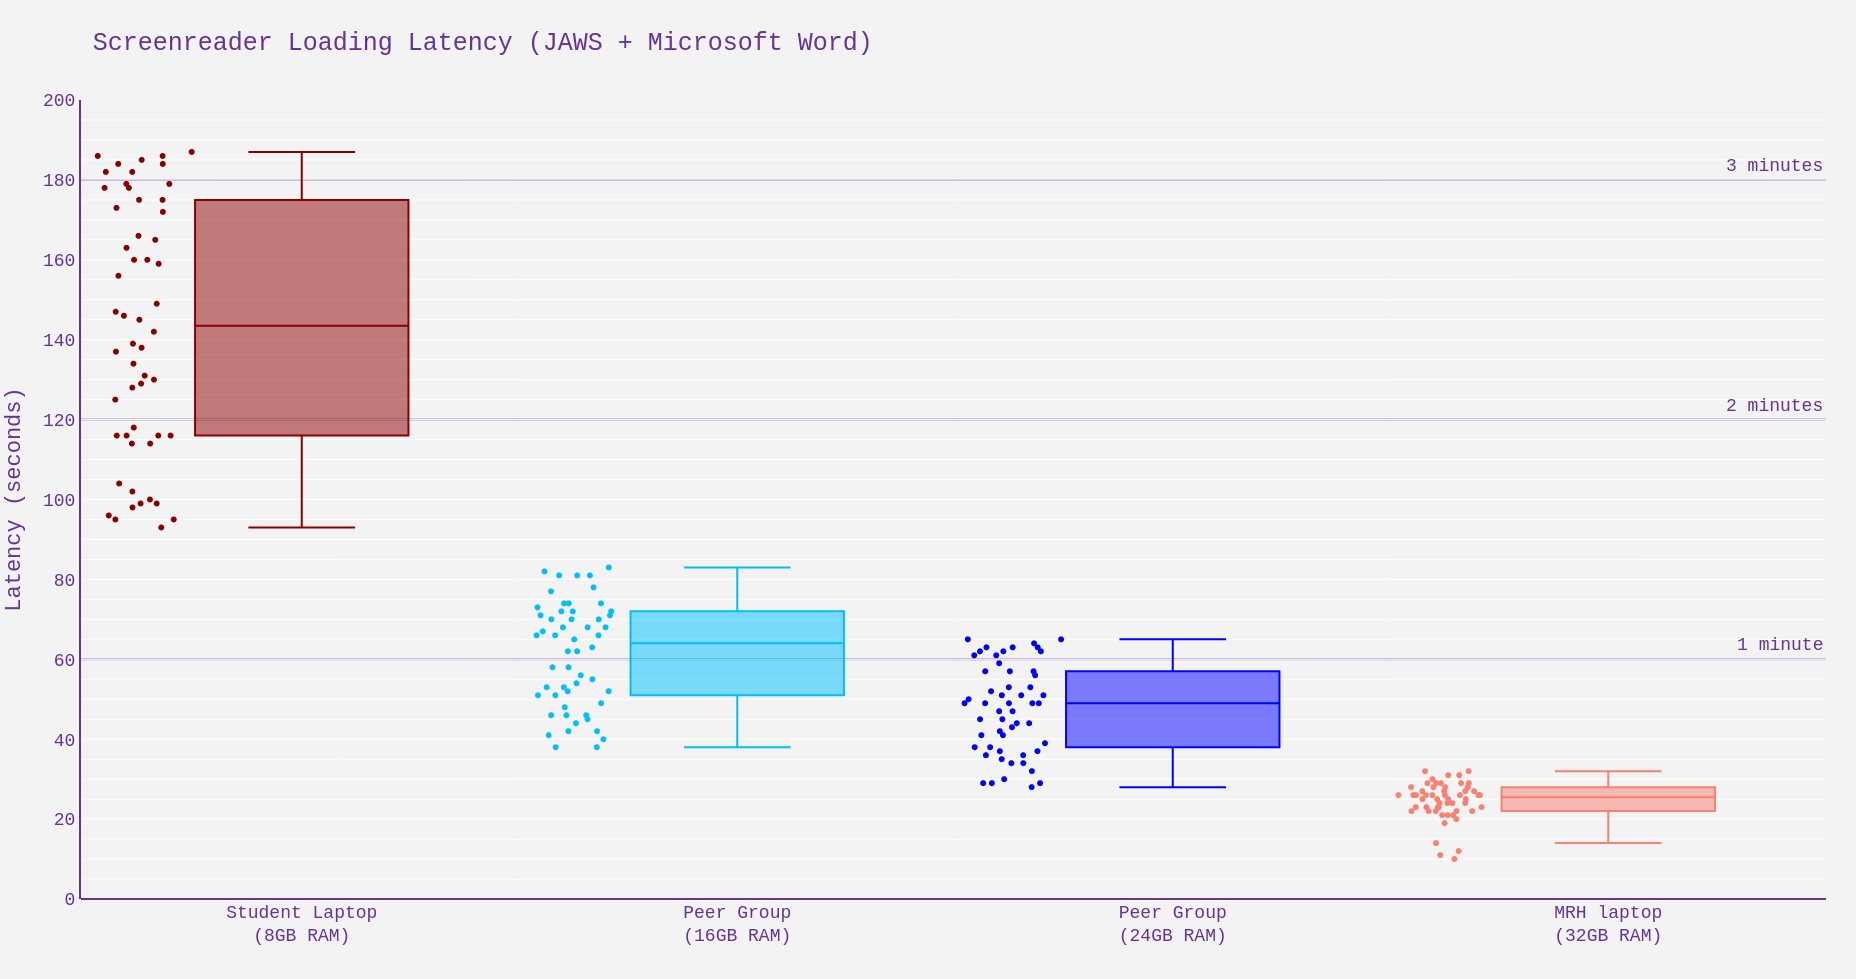
\includegraphics[width=\textwidth, alt={Boxplot of Screenreader loading latency for laptops with different amounts of RAM. A laptop with 8GB RAM took 143 seconds to load, 16GB took 64GB to load, 24GB RAM took 49 seconds to load, and 32GB RAM took 25 seconds to load}]{images/ComputerRBDisplaySpecsTVIFig1.png}
\caption[Latency to Load JAWS]{Plot showing Latency to Load JAWS while Microsoft Word is open across a typical student laptop (Dell Latitude 3190 with 8GB RAM), a high quality student laptop (Dell Precision 3530 with 16GB RAM), a professional laptop (Lenovo ThinkPad E16 with 24GB RAM), and a high power laptop (Microsoft Surface Laptop 3 with 32GB RAM).}\label{fig:figure1}
\end{figure}

\pagebreak
\hypertarget{screenreader-response}{}\section{Screenreader Responsiveness}\label{screenreader-response}
Measuring the latency of a screenreader to respond to key presses is important to determine if the laptop has sufficient RAM to run the software properly. If the laptop has insufficient RAM, the screenreader may take longer to respond to key presses, which can lead to delays in the user’s workflow. Measuring the latency of a screenreader can help identify if the laptop has enough RAM to run the software smoothly. This can help users avoid frustration and improve their productivity. Additionally, measuring the latency of a screenreader can help users identify if there are other issues with their laptop that may be causing the software to run slowly. By measuring the latency of a screenreader, users can ensure that their laptop is running optimally and that they are getting the most out of their software. \textit{Table \ref{tab:table5}} provides these data for the same computers shown in Figure \textit{\ref{fig:figure1}}.

\pagebreak\begin{longtable}[]{
>{\raggedright\arraybackslash}m{.5\textwidth}
>{\raggedright\arraybackslash}m{.25\textwidth}
>{\raggedright\arraybackslash}b{.25\textwidth}
}
\toprule
\textbf{Computer} \break (Color as Labelled in Figure 1) \\
\midrule
\endhead \hline \\
\multicolumn{3}{r}{\textbf{Continued on Next Page}} \endfoot
\endlastfoot
\fcolorbox{red}{red}{\rule{0pt}{6pt}\rule{6pt}{0pt}}\qquad $\begin{array}{l}\textbf{Students Laptop}\footnote{\raggedright Dell Latitude 3190} \\ \text{8GB RAM}\end{array}$ & 143 [93-183] \footnote{\raggedright These are the data plotted in Figure \ref{fig:figure1} above. The responsiveness data are more clear when presented as a table here than as a plot} & 38 [27-91]\footnote{\raggedright It is further important to note here that any lag in screenreader responsiveness of \textgreater1 sec means the student is behind their peers and their educational opportunity is limited by the technology not being sufficient (\emph{i.e.}, not an adequate accommodation). } \\ \cdashline{1-3}
\fcolorbox{cyan}{cyan}{\rule{0pt}{6pt}\rule{6pt}{0pt}}\qquad $\begin{array}{l}\textbf{Student/Professional Laptop}\fnsep\footnote{\raggedright Dell Precision 3530} \\ \text{16GB RAM}\end{array}$ & 64 [38-93] & 9 [4-15] \\ \cdashline{1-3}
\fcolorbox{violet}{violet}{\rule{0pt}{6pt}\rule{6pt}{0pt}}\qquad$\begin{array}{l}\textbf{Professional Laptop}\footnote{\raggedright Lenovo ThinkPad E16 (TVI Personal Laptop)} \\ \text{24GB RAM}\end{array}$ & 49 [26-65] & 1 [0.05-2.5] \\ \cdashline{1-3}
\fcolorbox{orange}{orange}{\rule{0pt}{6pt}\rule{6pt}{0pt}}\qquad$\begin{array}{l}\textbf{Professional Laptop}\footnote{\raggedright Microsoft Surface 3 (My Personal Laptop)} \\ \text{32GB RAM}\end{array}$ & 25 [10-32] & 0.5 [0.01-1]\footnote{\raggedright 0.01 represents an immediate response that could not be measured} \\ [1.0em] \hline \caption{Lag in JAWS Reporting Readable Content} \\
{\rule{0pt}{6pt}\rule{6pt}{0pt}}\qquad$\begin{array}{l}\textbf{Professional Laptop}\footnote{\raggedright Framework 16.0 (My Personal Laptop)} \\ \text{64GB RAM}\end{array}$ & XX [XX-XX] & XX.XX [XX-XX]\footnote{\raggedright 0.01 represents an immediate response that could not be measured} \\ [1.0em] \hline \caption{Lag in JAWS Reporting Readable Content}\label{tab:table5} \\
\end{longtable}

\pagebreak\hypertarget{laptop-RAM-use}{}\section{Measured Laptop RAM with Accessibility Tools}\label{laptop-RAM-use}
To demonstrate the actual RAM usage, I used a Dell Precision 3530 with 16GB RAM (second option in \textit{Table \ref{tab:table5}} and \textit{Figure \ref{fig:figure1}}\footnote{\raggedright This laptop has an integrated NVIDIA Quadro P600 GPU}) and the built-in snipping tool to measure RAM and CPU usage shown in the Activity monitor. \textit{Figure \ref{fig:figure2}} shows the results of this evaluation.

\textit{Figure \ref{subfig:figure2a}} shows RAM values for just the Windows 11 background Processes, \textit{Figure \ref{subfig:figure2b}} shows RAM usage with only JAWS screenreader added\footnote{\raggedright The previous addition was turned off and the computer restarted prior to each test and the system allowed to reach equilibrium for 3 minutes prior to taking any screenshots}, \textit{Figure \ref{subfig:figure2c}}, shows RAM usage with ZoomText magnification, and finally \textit{Figure \ref{subfig:figure2d}}, shows RAM usage with Freedom Scientific Fusion (Integrated JAWS + ZoomText). I use these options as they are considered the gold standard and are industry standard.

\begin{figure}[H]
\centering
\subfloat[Background RAM Usage - 7.7GB]{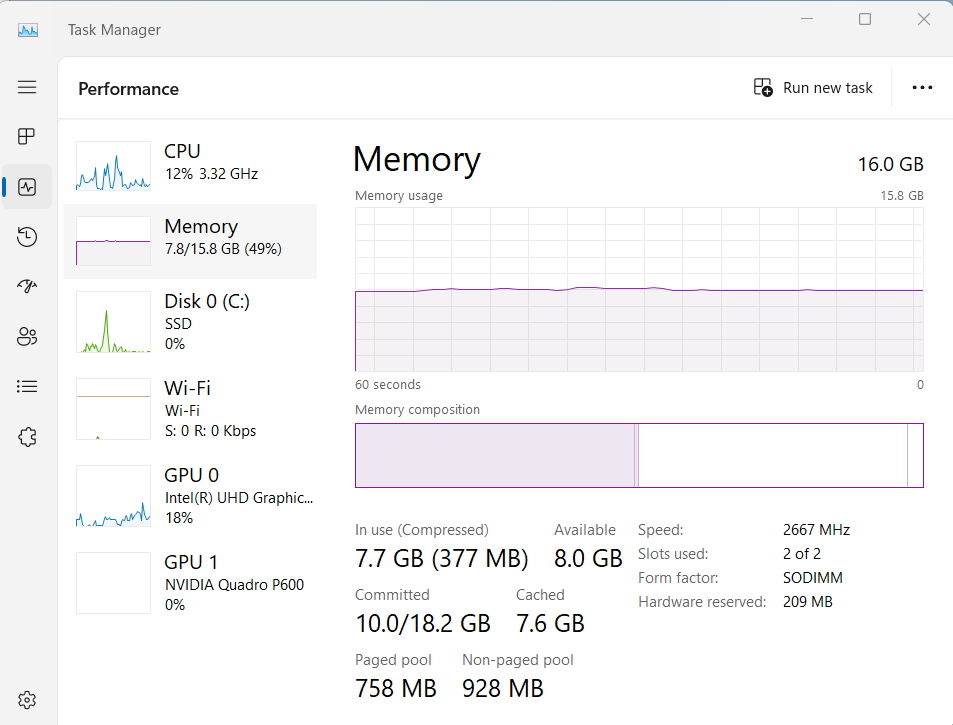
\includegraphics[width=.48\textwidth, alt={Screenshot of Activity Monitor showing 7.7GB RAM with no NVIDIA GPU usage, and 12\% CPU used}]{images/NOTHING.png}\label{subfig:figure2a}}
\hfill
\subfloat[RAM Usage JAWS - 9.9GB]{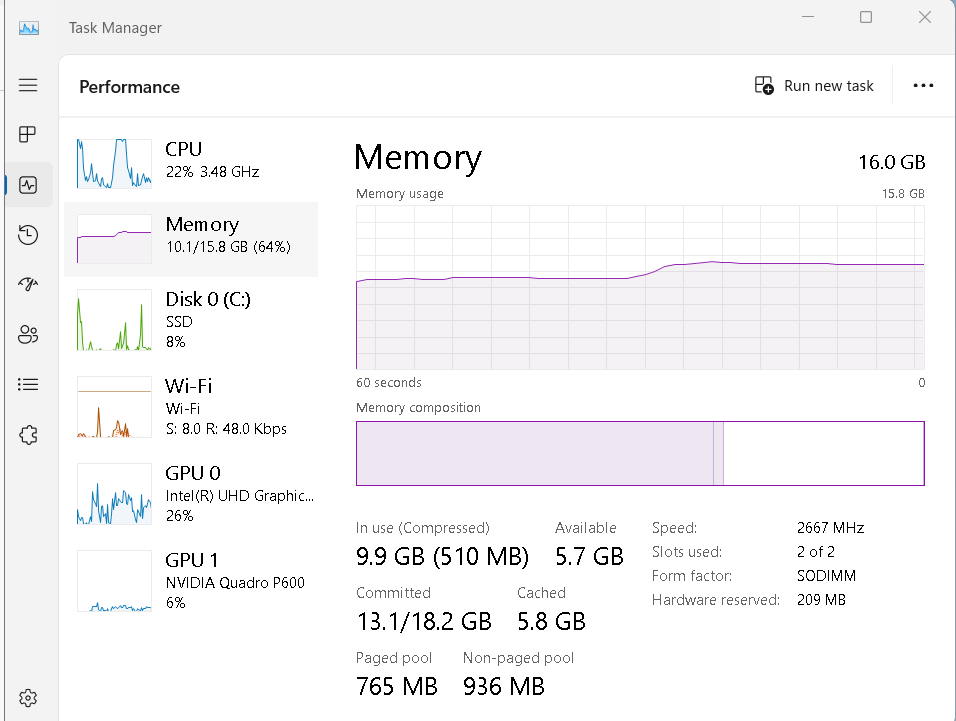
\includegraphics[width=0.48\textwidth, alt={Screenshot of Activity Monitor showing 9.9GB RAM with 6\% NVIDIA GPU usage, and 22\% CPU used}]{images/JAWS.png}\label{subfig:figure2b}}
\hfill\\
\subfloat[RAM Usage ZoomText - 11.0GB]{\includegraphics[width=0.48\textwidth, alt={Screenshot of Activity Monitor showing 12.7GB RAM with 6\% NVIDIA GPU usage (and GPU temp of 65 \textdegree C), and 100\% CPU used}]{images/ZoomText.png}\label{subfig:figure2c}}
\hfill
\subfloat[RAM Usage Fusion - 13.8GB]{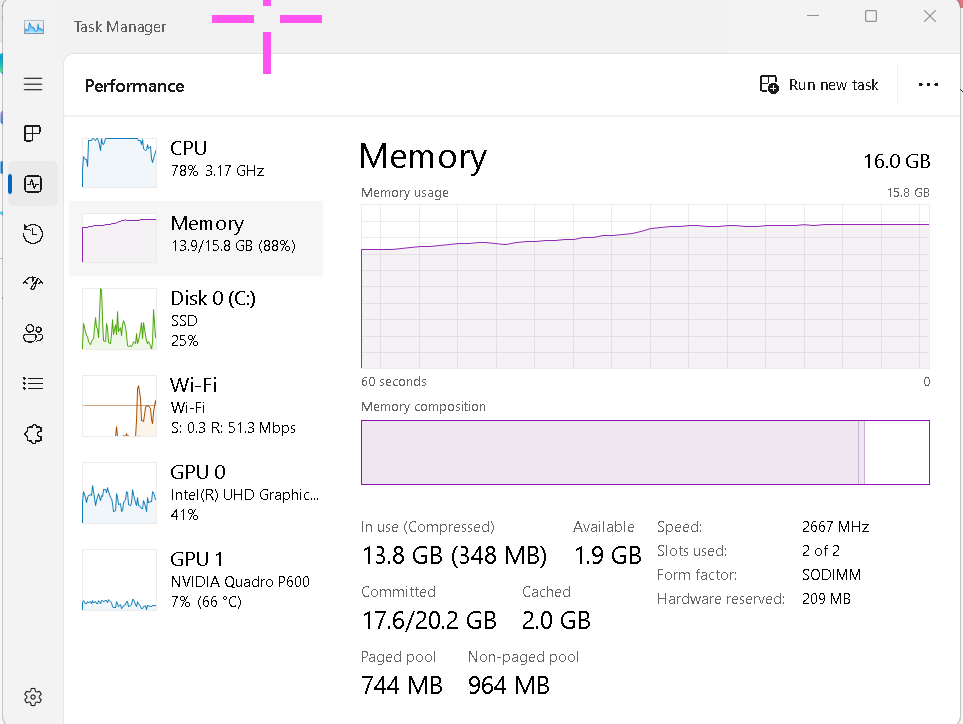
\includegraphics[width=.48\textwidth, alt={Screenshot of Activity Monitor showing 12.7GB RAM with 7\% NVIDIA GPU usage (and GPU temp of 66\textdegree C), and 78\% CPU used}]{images/FUSION_final.png}\label{subfig:figure2d}}
\caption[Measured Laptop RAM with only Accessibility Tools Open]{Measured Laptop RAM with only Accessibility Tools Open.  Note that this laptop has two GPU, GPU0 is the Intel® Videos card and GPU1 is an NVIDIA Quadro P600, both of which show much less activity in this test than the next one shown in Figure \ref{fig:figure3}}
\label{fig:figure2}
\end{figure}

\newpage \textit{Figure \ref{fig:figure3}} shows measures laptop RAM with the same laptop as used in \textit{Figure \ref{fig:figure2}}. \textit{Figure \ref{subfig:figure3a}} shows RAM usage with JAWS and Word running, \textit{Figure \ref{subfig:figure3b}} ZoomText + Word, and \textit{Figure \ref{subfig:figure3c}} Fusion and Microsoft Word running in the background.

\begin{figure}[H]
\centering
\subfloat[RAM Usage JAWS + Word - 10.7GB]{\hfill 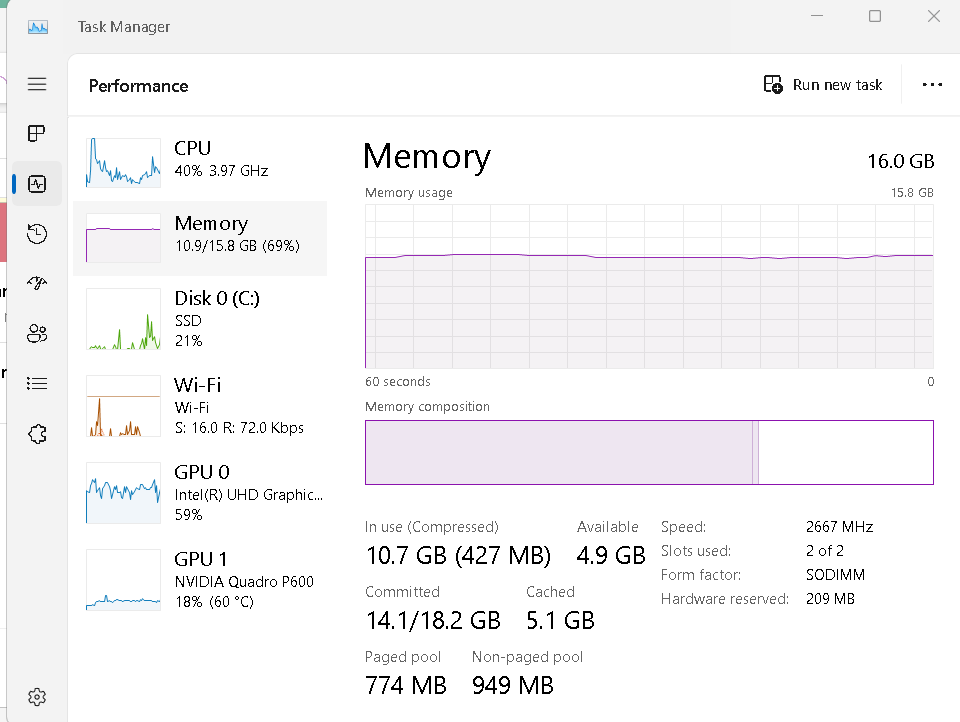
\includegraphics[width=.6\textwidth, alt={Screenshot of Activity Monitor showing 10.7GB RAM with 18\% NVIDIA GPU usage (and GPU temp of 60\textdegree C), and 40\% CPU used}]{images/JAWS+WORD.png}\label{subfig:figure3a}} \\   \hfill
\subfloat[RAM Usage ZoomText + Word - 14.5GB]{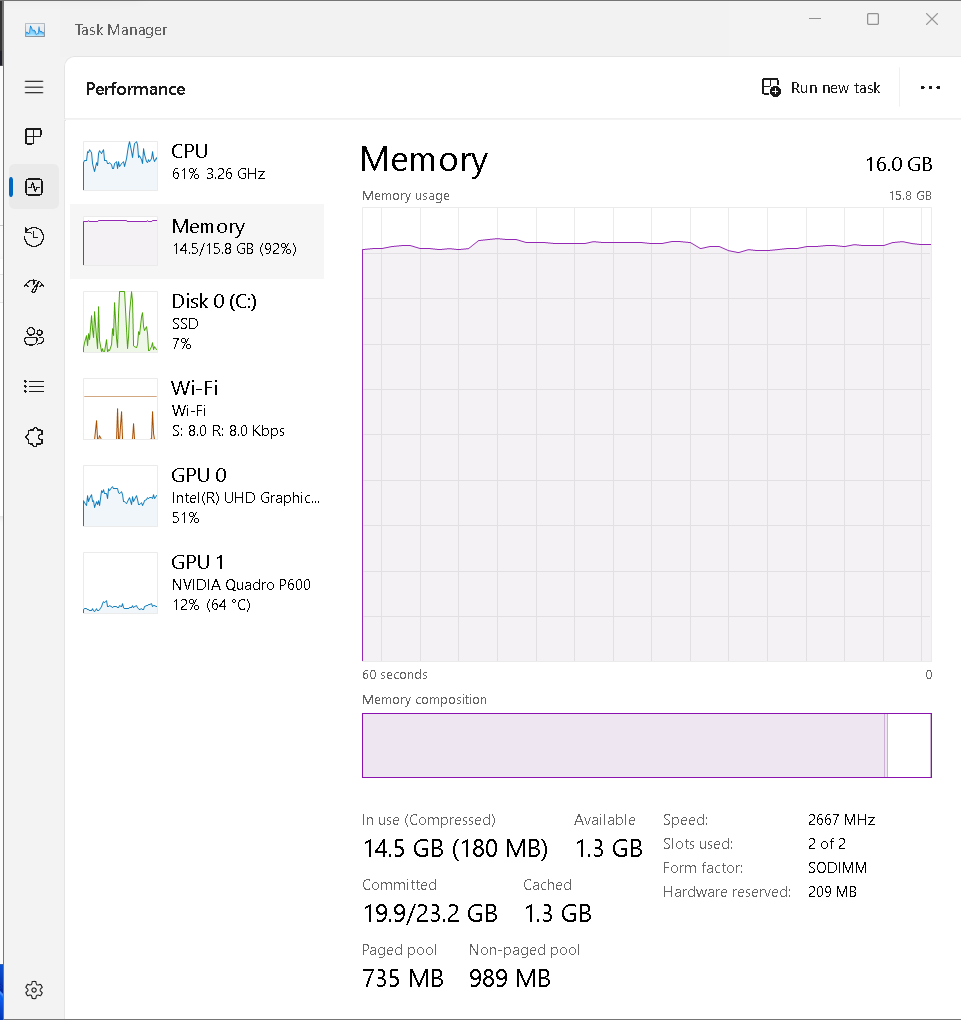
\includegraphics[width=0.45\textwidth, alt={Screenshot of Activity Monitor showing 14.5GB RAM with 12\% NVIDIA GPU usage (and GPU temp of 64\textdegree C), and 61\% CPU used}]{images/ZoomTEXT+WORD.png}\label{subfig:figure3b}}
\hfill
\subfloat[RAM Usage Fusion + Word - 14.8GB]{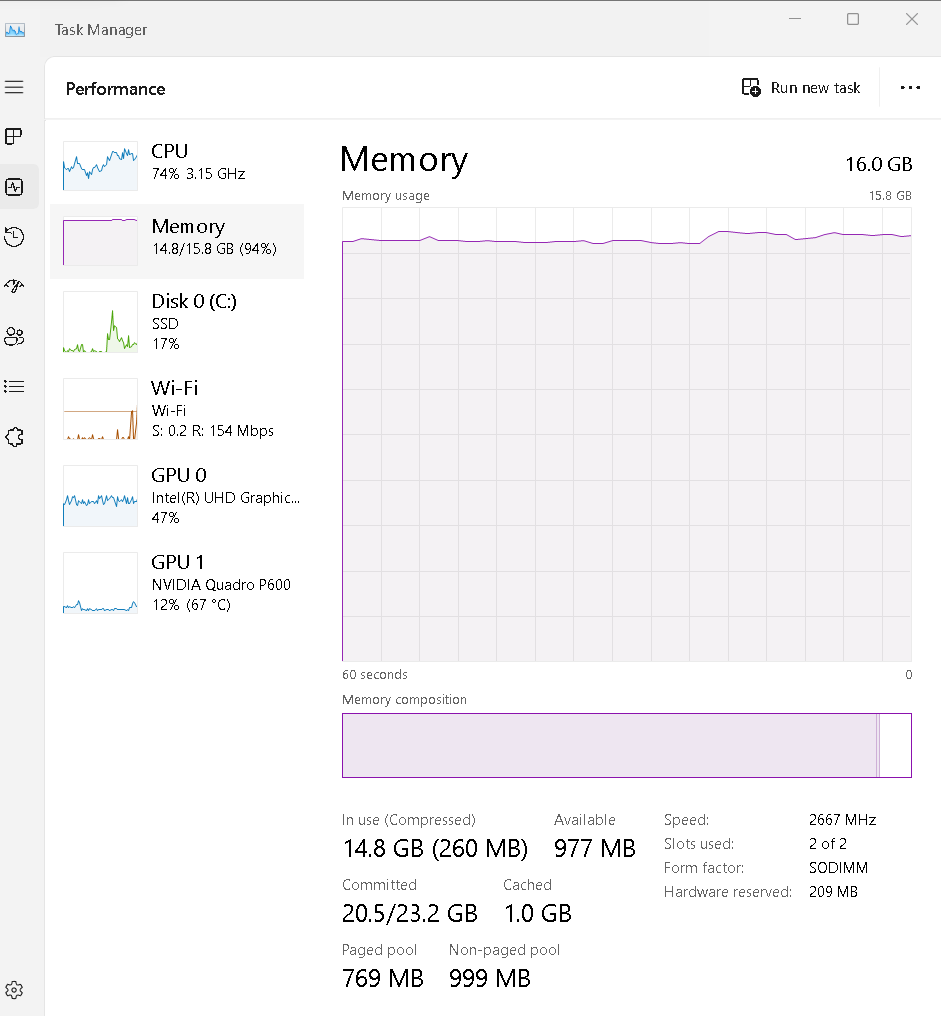
\includegraphics[width=0.45\textwidth, alt={Screenshot of Activity Monitor showing 12.7GB RAM with 12\% NVIDIA GPU usage (and GPU temp of 67\textdegree C), and 74\% CPU used}]{images/FUSION+WORD.png}\label{subfig:figure3c}}
\caption[Measured Laptop RAM with Accessibility Tools + Microsoft Word]{Measured Laptop RAM with Accessibility Tools + Microsoft Word. Note that this laptop has two GPU, GPU0 is the Intel® Videos card and GPU1 is an NVIDIA Quadro P600, both of which show much higher activity in this test than the previous shown in Figure \ref{fig:figure2}}
\label{fig:figure3}
\end{figure}

\pagebreak \hypertarget{notes-on-future-proofing-laptops}{}\section{Laptop Cost Factors}\label{notes-on-future-proofing-laptops}
Students with visual impairments require laptops that are compatible with assistive technology to receive a free and accessible public education. When selecting a laptop, there are several cost factors that must be taken into account. Firstly, the laptop should have sufficient RAM to run the assistive technology software smoothly. Secondly, the laptop should have a high-quality screen that is large enough to display text and images clearly. Thirdly, the laptop should have a long battery life to ensure that students can use it for extended periods of time without needing to recharge. Fourthly, the laptop should have a durable build quality to withstand daily wear and tear. Finally, the laptop should be lightweight and portable to enable students to carry it around easily. These factors can help ensure that students with visual impairments have access to the technology they need to succeed in their studies.

\hypertarget{future-proofing}{}\subsection{Laptop Durability}\label{future-proofing}

I asked ChatGPT why we should consider future usage needs of a laptop into my purchasing plans and here is its response (emphasis mine):

\begin{leftbar} \begin{quote}
Buying laptops with high-end RAM and processor specifications can be beneficial for several reasons, especially in terms of longevity and performance. Here are some key considerations:

\begin{enumerate}[leftmargin=*]
\def\labelenumi{\arabic{enumi}.}

\item
Future-Proofing:
\end{enumerate}

\begin{itemize}

\item
Investing in higher-end components can help future-proof your laptop to some extent. As software and applications become more demanding over time, a laptop with better specifications is likely to remain relevant and capable of handling new software updates and requirements.
\end{itemize}

\begin{enumerate}[leftmargin=*]
\def\labelenumi{\arabic{enumi}.}
\setcounter{enumi}{1}

\item
Multitasking and Performance:
\end{enumerate}

\begin{itemize}

\item
Higher RAM allows for better multitasking capabilities. If you use resource-intensive applications or run multiple programs simultaneously, having ample RAM prevents slowdowns and ensures smooth performance.
\item
A powerful processor can handle complex computations and tasks more efficiently, contributing to faster overall system performance.
\end{itemize}

\begin{enumerate}[leftmargin=*]
\def\labelenumi{\arabic{enumi}.}
\setcounter{enumi}{2}

\item
Graphics Processing:
\end{enumerate}

\begin{itemize}

\item
For tasks such as video editing, gaming, or other graphics-intensive applications, a high-end GPU (Graphics Processing Unit) is crucial. This is separate from RAM and the main processor but is equally important for certain tasks.
\end{itemize}

\begin{enumerate}[leftmargin=*]
\def\labelenumi{\arabic{enumi}.}
\setcounter{enumi}{3}

\item
Long-Term Usability:
\end{enumerate}

\begin{itemize}

\item
Technology advances quickly, and what is considered high-end today might become standard or entry-level in a few years. However, starting with a high-end laptop gives you a more extended period before your system becomes outdated.
\end{itemize}

\begin{enumerate}[leftmargin=*]
\def\labelenumi{\arabic{enumi}.}
\setcounter{enumi}{4}

\item
Smooth Upgrades:
\end{enumerate}

\begin{itemize}

\item
Some laptops allow users to upgrade certain components like RAM and storage. Starting with higher-end specifications provides more headroom for future upgrades, allowing you to extend the useful life of your laptop.
\end{itemize}

\begin{enumerate}[leftmargin=*]
\def\labelenumi{\arabic{enumi}.}
\setcounter{enumi}{5}

\item
Resource-Intensive Applications:
\end{enumerate}

\begin{itemize}

\item
If you use applications that require a lot of processing power, like video editing software, 3D modeling tools, or virtualization software, a high-end laptop can handle these tasks more efficiently, providing a better user experience.
\end{itemize}

\begin{enumerate}[leftmargin=*]
\def\labelenumi{\arabic{enumi}.}
\setcounter{enumi}{6}

\item
Responsiveness and Speed:
\end{enumerate}

\begin{itemize}

\item
A faster processor and more RAM contribute to a more responsive system. Applications load quicker, and the overall user experience is smoother, which can significantly impact productivity.
\end{itemize}

\begin{enumerate}[leftmargin=*]
\def\labelenumi{\arabic{enumi}.}
\setcounter{enumi}{7}

\item
Enhanced Resale Value:
\end{enumerate}

\begin{itemize}

\item
High-end laptops generally retain their value better than lower-end models. If you decide to sell or upgrade your laptop in the future, having top-tier specifications can make it more attractive to potential buyers.
\end{itemize}

It's important to note that the specific requirements depend on your usage patterns and needs. Not everyone needs the highest specifications, and sometimes a mid-range laptop can be more than sufficient for everyday tasks. However, \textbf{for users with demanding workloads or those who want a longer usable life from their device, opting for higher-end specifications can be a wise investment}.
\end{quote}\end{leftbar}

\pagebreak \hypertarget{gpu-needs}{}\subsection{Role of GPU in Laptop Performance}\label{gpu-needs}
A CPU or Central Processing Unit is the primary processor of a computer. It is responsible for executing instructions and performing calculations for all the programs running on the computer. A GPU or Graphics Processing Unit, on the other hand, is a specialized processor designed to handle complex calculations required for rendering graphics and images. While a CPU is designed to handle a wide range of tasks quickly, a GPU is designed to quickly render high-resolution images and video concurrently\footnote{\raggedright \href{https://www.weka.io/learn/gpu/what-is-a-gpu/}{WekaIO. (n.d.). What is a GPU? WekaIO}}.

When it comes to improving laptop performance for graphics-intensive tasks or coding, a dedicated GPU can significantly improve performance. A dedicated GPU is a separate processor that is designed to handle the complex calculations required for rendering graphics and images. By offloading the processing of graphics data from the CPU, a dedicated GPU allows the CPU to focus on other tasks, resulting in faster and smoother performance for graphics-intensive applications. Additionally, a GPU can also be beneficial for processes involving AI. AI algorithms require a lot of processing power, and a GPU can help speed up the process. NVIDIA®,  AMD®,  and Intel® are some of the most popular GPU manufacturers, with models available for both desktop and laptop computers. Laptops with a dedicated GPU can handle AI tasks with ease, making them ideal for professionals who work with AI\footnote{\raggedright \href{https://www.reddit.com/r/framework/comments/14pb7b/outside_of_videogames_what_is_the_point_of_a/}{u/ChaosMotor: Outside of videogames, what is the point of a "framework"? (2012, December 12). Reddit}}.

In summary, a CPU is responsible for executing instructions and performing calculations for all the programs running on the computer, while a GPU is a specialized processor designed to handle complex calculations required for rendering graphics and images\footnotemark[52]. A dedicated GPU can significantly improve laptop performance for graphics-intensive tasks such as gaming, video editing, and 3D modeling by offloading the processing of graphics data from the CPU. Screen magnification software can also benefit from a dedicated GPU. Screen magnification software enlarges the content on the screen, which can be taxing on the CPU. A dedicated GPU can help alleviate this burden by handling the graphics processing required for screen magnification. This results in a smoother and more responsive experience when using screen magnification software\footnote{\raggedright \href{https://www.run.ai/guides/multi-gpu/cpu-vs-gpu}{Run:AI. (n.d.). CPU vs GPU: Architecture, Pros and Cons, and Special Use Cases. Run:AI}}.

I evaluated with my personal laptop\footnote{\raggedright My 4 year-old Surface Laptop 3 at the time of the evalutaion} the role for a CPU and GPU in using screenreader and magnification software. I also did the same with the mid-range professional laptop with 16GB of RAM. I found there was no increase in performance for JAWS, ZDSR, NVDA, or Dolphin Screenreader when an integrated GPU was present (AMD® Vega® 10 or Intel® UHD Graphics 630 integrated GPU). However, when I assessed performance of ZoomText, Fusion (ZoomText + JAWS), and Dolphin SuperNova magnifier, as well as Dolphin Magnifier + ScreenReader, I saw a 30-45\% increase in responsiveness for both speech and visual markers available on the screen. In this case I opened 10 tabs in Google Chrome, 10 tabs in Microsoft Edge, 10 tabs in Mozilla Firefox, and started typing in an online Microsoft Word document using office 365 online. Response time refers to the time it took the system to react when I typed beyond the field of view and the system had to move the screen and visual screen marker to a new location. \textit{Table \ref{tab:table51}} shows these data. Importantly, both of the laptops were able to improve their performance for Magnification tasks by a similar percentage when the integrated GPU was used in concert with the CPU.

\pagebreak\begin{longtable}[]{
>{\raggedright\arraybackslash}m{.4\textwidth}
>{\raggedright\arraybackslash}m{.25\textwidth}
>{\raggedright\arraybackslash}m{.25\textwidth}
>{\raggedright\arraybackslash}m{.1\textwidth}
}
\toprule
& \multicolumn{2}{c}{\textbf{Latency (s)}} & \\ \cline{2-3}
& \textbf{CPU} & \textbf{CPU+GPU} & \textbf{\% Faster} \\
\midrule
\endhead \hline \\
\multicolumn{2}{r}{\textbf{Continued on Next Page}} \endfoot
\endlastfoot
\multicolumn{2}{l}{\textbf{Screenreader Only}\footnote{\raggedright The visual marker outlining the current focus was used to measure response}} \\
JAWS Screenreader & $\begin{array}{l}0.5~~[0.01-1] \\9.0~~[4-15]\end{array}$ & $\begin{array}{l}0.5~~[0.01-1] \\9.0~~[3-17]\end{array}$ & $\begin{array}{l} 0\% \\ 0\%\end{array}$ \\ \cdashline{2-4}
JAWS Screenreader & $\begin{array}{l}0.5~~[0.01-1] \\9.0~~[4-15]\end{array}$ & $\begin{array}{l}0.5~~[0.01-1] \\9.0~~[3-17]\end{array}$ & $\begin{array}{l} 0\% \\ 0\%\end{array}$ \\ \cdashline{2-4}
NVDA Screenreader & $\begin{array}{l}0.2~~[0.01-0.5] \\4.0~~[1.5-6]\end{array}$ & $\begin{array}{l}0.2~~[0.01-0.5] \\4.0~~[1.5-6]\end{array}$ & $\begin{array}{l} 0\% \\ 0\%\end{array}$ \\ \cdashline{2-4}
Dolphin Screenreader & $\begin{array}{l}0.5~~[0.01-1] \\9.0~~[5-17]\end{array}$ & $\begin{array}{l}0.5~~[0.01-1] \\8.8~~[5-17]\end{array}$ & $\begin{array}{l} 0\% \\ 2\%\end{array}$ \\ \cdashline{2-4}
ZDSR Screenreader & $\begin{array}{l}0.2~~[0.01-0.75] \\5.0~~[2-7]\end{array}$ & $\begin{array}{l}0.2~~[0.01-0.75] \\5.0~~[2-7]\end{array}$ & $\begin{array}{l} 0\% \\ 0\%\end{array}$ \\ \cdashline{2-4}
\multicolumn{2}{l}{\textbf{Screen Magnification Only}\footnotemark[48]} \\
ZoomText & $\begin{array}{l}1.1~~[0.5-1.25] ] \\15~~~[10-19]\end{array}$ & $\begin{array}{l}.75~~[0.3-1] ] \\5~~~~~[2.5-10]\end{array}$ & $\begin{array}{l} 32\% \\ 33\%\end{array}$ \\ \cdashline{2-4}
SuperNova & $\begin{array}{l}1.5~~[0.75-1.45] \\11~~~[4-20]\end{array}$ & $\begin{array}{l}.77~~[0.4-1] \\7~~~~~[3-11]\end{array}$ & $\begin{array}{l} 48\% \\ 36\%\end{array}$ \\ \cdashline{2-4}
\multicolumn{2}{l}{\textbf{Screenreader + Magnification}\footnotemark[48]} \\
SuperNova + Magnification & $\begin{array}{l}1.5~~[1-25] ] \\16~~~[9-25]\end{array}$ & $\begin{array}{l}.75~~[0.25-1] ] \\6~~~~~[3-15]\end{array}$ & $\begin{array}{l} 48\% \\ 37\%\end{array}$ \\ \cdashline{2-4}
Fusion (ZoomText + JAWS) & $\begin{array}{l}1.5~~[1-1.75] \\13~~~[3-19]\end{array}$ & $\begin{array}{l}.75~~[0.25-1] \\5~~~~~[2.5-13]\end{array}$ & $\begin{array}{l} 48\% \\ 38\%\end{array}$ \\[1.0em]\hline
\caption[Screen Magnifiers Benefit from Integrated GPU]{Screen Magnifiers Benefit from Use of an Integrated GPU. The top row in each table cell contains data for the laptop with 32GB RAM, an AMD® Ryzen™ 7 processor and AMD® Vega™  10 integrated GPU. The lower crow in each cell contains data for the laptop with 16GB RAM, an 8th Gen 17 processor, and Intel® UHD 630 integrated GPU. Integrated GPU were activated or inactivated by turning hardware acceleration ON or OFF for each laptop} \label{tab:table51}
\end{longtable}

\pagebreak \hypertarget{optimizing-cost-with-performance}{}\subsection{Laptop Cost Optimization}\label{optimizing-cost-with-performance}

There is an economic theory based on a Terry Pratchett novel that explains this phenomenon better than we can. It is called the \href{http://en.wikipedia.org/wiki/Boots_theory}{Vimes Boots Index}\footnote{\raggedright Full Text (emphasis mine):
\begin{leftbar}
\begin{quote}The reason that the rich were so rich, Vimes reasoned, was because they managed to spend less money.

Take boots, for example. He earned thirty-eight dollars a month plus allowances. A really good pair of leather boots cost fifty dollars. But an affordable pair of boots, which were sort of OK for a season or two and then leaked like hell when the cardboard gave out, cost about ten dollars. Those were the kind of boots Vimes always bought, and wore until the soles were so thin that he could tell where he was in Ankh-Morpork on a foggy night by the feel of the cobbles.

But the thing was that good boots lasted for years and years. \textbf{A man who could afford fifty dollars had a pair of boots that’d still be keeping his feet dry in ten years’ time, while the poor man who could only afford cheap boots would have spent a hundred dollars on boots in the same time and would still have wet feet.}

Basically, \textbf{we are destined to be stuck in a cycle of perpetually spending more money for inferior products and will, in the end, spend more money than if we just paid for better product in the first place.} \break \qquad-- \textit{Men At Arms}, page 38
\end{quote}
\end{leftbar}
}

\hfill \break \textit{Table \ref{tab:table6}} illustrates this theory in terms of student laptop computers (Assuming student has a laptop using a screenreader through 3rd-12th grade). \textit{Table \ref{tab:table6}} also illustrates why we choose to err on the side of spending \$2000-3000 on a laptop computer that will last 3-5 years over spending \$1500-2000 on a laptop that will reach end-of-life within 1-2 years before becoming obsolete. By the end of 5 years we will have spent more on Low End and Mid Range Laptops than we would have otherwise spent had we purchased a High End Laptop. Importantly; however, we also would have been using laptops that always performed more poorly than a High End laptop would.

\pagebreak\begin{longtable}[]{
>{\raggedright\arraybackslash}m{.15\textwidth}
>{\raggedright\arraybackslash}m{.05\textwidth}
>{\raggedright\arraybackslash}m{.05\textwidth}
>{\raggedright\arraybackslash}m{.05\textwidth}
>{\raggedright\arraybackslash}m{.05\textwidth}
>{\raggedright\arraybackslash}m{.05\textwidth}
>{\raggedright\arraybackslash}m{.05\textwidth}
>{\raggedright\arraybackslash}m{.05\textwidth}
>{\raggedright\arraybackslash}m{.05\textwidth}
>{\raggedright\arraybackslash}m{.05\textwidth}
>{\raggedright\arraybackslash}m{.05\textwidth}
>{\raggedright\arraybackslash}b{.10\textwidth}
}
\toprule & \multicolumn{10}{c}{\textbf{Does School Have to Purchase a Replacement Laptop by Year}} & \\ \cdashline{1-12}
\cline{2-11} \\
\textbf{RAM} \break Cost & \textbf{1} & \textbf{2} & \textbf{3} & \textbf{4} & \textbf{5} & \textbf{6} & \textbf{7} & \textbf{8} & \textbf{9} & \textbf{10} & \textbf{10-year Cost} \\
\midrule
\endhead \hline \\
\multicolumn{6}{r}{\textbf{Continued on Next Page}} \endfoot
\endlastfoot
\textbf{4GB}\footnote{\raggedright Dell Latitude 3190 Education}\fnsep\footnote{\raggedright The 4GB Laptop \textit{cannot} run JAWS and is included to show price comparison to the other options} \break \$525 & $\checkmark$ & $\checkmark$ & $\checkmark$ & $\checkmark$ & $\checkmark$ & $\checkmark$ & $\checkmark$ & $\checkmark$ & $\checkmark$ & $\checkmark$ & \$1250 \\ \cdashline{1-12}
\textbf{4GB}\footnote{\raggedright Lenovo 500w Gen 3 Education}\fnsep\footnotemark[59] \break \$550 & $\checkmark$ & $\checkmark$ & $\checkmark$ & $\checkmark$ & $\checkmark$ & $\checkmark$ & $\checkmark$ & $\checkmark$ & $\checkmark$ & $\checkmark$ & \$1500 \\ \cdashline{1-12}
\textbf{8GB}\footnote{\raggedright Dell Latitude 3190 Education} \break \$1184 & $\checkmark$ & $\checkmark$ & $\checkmark$ & $\checkmark$ & $\checkmark$ & $\checkmark$ & $\checkmark$ & $\checkmark$ & $\checkmark$ & $\checkmark$ & \$11,840 \\ \cdashline{1-12}
\textbf{16GB}\footnote{\raggedright Dell Precision 3530 given to TVIs teaching screenreaders} \break \$1751 & $\checkmark$ & - & $\checkmark$ & - & $\checkmark$ & - & $\checkmark$ & - & $\checkmark$ & - & \$1755 \\ \cdashline{1-12}
\textbf{32GB}\footnote{\raggedright Microsoft Surface Laptop 3}\break \$2824\break \textcolor{red}{\textit{\textbf{Best Case}}}\footnote{\raggedright This is my personal experience} & $\checkmark$ & - & - & - & - & $\checkmark$ & - & - & - & - & \$1648 \\ \cdashline{1-12}
\textbf{32GB}\footnote{\raggedright Microsoft Surface Laptop 3}\break \$2824\break \textcolor{red}{\textit{\textbf{Cautious}}}\footnote{\raggedright This is a conservative estimate to account for potential rough treatment of a computer} & $\checkmark$ & - & - & $\checkmark$ & - & - & $\checkmark$ & - & - & - & \$1472 \\[1.0em]\hline
\caption[Cost of Laptops over Time]{Cost of Laptops Across Time. Notice that the final cost of the 32GB option is comparable to the 4GB options over 10 years. However, the 4GB laptops are not capable of running JAWS reliably in the classroom setting.
\break\textbullet For the \textcolor{red}{\textbf{Best Case}} Scenario, the 32GB laptop is between \$1107 and \$1192 \textit{\textbf{cheaper}} over time compared to the 16GB and 8GB laptops, respectively.
\break\textbullet For the \textcolor{red}{\textbf{Cautious}} Scenario, the 32GB laptop is between \$283 and \$1386 \textit{\textbf{cheaper}} over time compared to the 16GB and 8GB laptops, respectively}\label{tab:table6}
\end{longtable}

\pagebreak \hypertarget{timelineofreplacement}{}\subsection{Replacement Timeline}\label{timelineofreplacement}

Optimally, given the needs of students for use of technology in the classroom, the following timeline for laptop replacement is suggested\footnote{\raggedright this is based on the assumption of the school LEA and not the vision department being the first resource for purchasing technology}. The idea behind this timeline if to minmize the number of times any single LEA has to purchase a laptop for a student.

The student be provided with a laptop capable of screenreader usage in 3rd/4th grade depending upon the needs of the student. A replacement laptop should be provided in 7th grade when the student moves to middle school. A final replacement should be provided in 10th grade when the student moves to high school. This means during the 10 years of a student's education, the district would only have to purchase 3 laptops for the student, and each school would only have to purchase one.

To implement this plan, it is imperative that the vision team be involved in the decision making process for the laptop purchase, primarily to describe the software and hardware specifications required to meet each individual student's needs. This will ensure that the laptop is capable of running the necessary software for the student's entire educational career. These discussions need to start in December of the year previous to the purchasing of the laptop, so that the cost of the technology can be included in the school's technology budget for the following year and the STS can have time to determine which of any agreed upon laptop options fit both the needs of the student as well as the budgetary constraints of the school. This means that discussions should happen in December of the student's 2nd/3rd grade year (this depends upon when the students in that school move from an iPad based setup to using laptop computers), December of their 6th grade year with the middle school, and December of their 9th grade year with the high school.

\pagebreak
\hypertarget{minimum-laptop-recommendations}{}\section{Recommended Laptop Specifications}\label{minimum-laptop-recommendations}
\textit{Table \ref{tab:table7}} is a list of recommendations for laptop specifications by use case.

\pagebreak\begin{longtable}[]{
>{\raggedright\arraybackslash}m{.7\textwidth}
>{\raggedright\arraybackslash}b{.3\textwidth}
}
\toprule

\textbf{Use Case} & \textbf{Recommendation} \\
\midrule
\endhead \hline \\
\multicolumn{2}{r}{\textbf{Continued on Next Page}} \endfoot
\endlastfoot
\multicolumn{2}{l}{\textbf{Screenreader Only}} \\[1em]
JAWS Screenreader & \textgreater16GB \\ \cdashline{1-2}
NVDA Screenreader & \textgreater16GB \\ \cdashline{1-2}
Dolphin Screenreader & \textgreater16GB \\ \cdashline{1-2}
ZDSR Screenreader & \textgreater16GB \\ \cdashline{1-2}
\multicolumn{2}{l}{\textbf{Screen Magnification Only}\footnote{can also benefit from either an integrated or dedicated GPU}} \\[1em]
ZoomText & \textgreater24-32GB \\ \cdashline{1-2}
Windows Magnifier & \textgreater16GB \\ \cdashline{1-2}
Dolphin SuperNova & \textgreater24-32GB \\ \cdashline{1-2}
\multicolumn{2}{l}{\textbf{Screenreader + Magnification}\footnotemark[\value{footnote}]} \\[1em]
JAWS Screenreader + Windows Magnifier & \textgreater24-32GB \\ \cdashline{1-2}
NVDA Screenreader + Windows Magnifier & \textgreater24-32GB \\ \cdashline{1-2}
ZDSR Screenreader + Windows Magnifier & \textgreater24-32GB \\ \cdashline{1-2}
Dolphin Screenreader + Windows Magnifier & \textgreater24-32GB \\ \cdashline{1-2}
SuperNova Screenreader + Magnification & \textgreater32-64GB \\ \cdashline{1-2}
Fusion Screenreader + Magnification & \textgreater32-64GB \\\hline
\caption{Recommended Laptop Specifications}\label{tab:table7}
\end{longtable}

\pagebreak
\hypertarget{laptops-meeting-recommended-specifications}{}\section{Laptops Meeting Specifications}\label{laptops-meeting-recommended-specifications}
\textit{Table \ref{tab:table8}} is an alphabetical list of laptop computers that meet the recommended specifications defined in \textit{Table \ref{tab:table7}}.

\pagebreak\begin{longtable}[]{
>{\raggedright\arraybackslash}m{.35\textwidth}
>{\raggedright\arraybackslash}m{.12\textwidth}
>{\raggedright\arraybackslash}m{.12\textwidth}
>{\raggedright\arraybackslash}m{.12\textwidth}
>{\raggedright\arraybackslash}b{.2\textwidth}
}
\toprule
\textbf{Company / Model} & \textbf{Cost} & \textbf{RAM} & \textbf{Display} & \textbf{Processor} \\
\midrule
\endhead \hline \\
\multicolumn{5}{r}{\textbf{Continued on Next Page}} \endfoot
\endlastfoot
\multicolumn{5}{l}{\textbf{Screenreader Only\footnote{\raggedright Laptops without integrated/dedicated GPU units}}} \\ \cdashline{1-5}
\multicolumn{5}{l}{\break\textbf{\qquad\textless\$1000-\$2000}} \\ \cdashline{1-5}
Acer Aspire 5 & \$1319 & 32GB & 15.6 & 13th Gen Intel® Core™ i7 \\ \cdashline{1-5}
Acer Swift Go 16 & \$999 & 32GB & 14.0 & 13th Gen Intel® Core™ i7 \\ \cdashline{1-5}
ASUS Vivobook 17X & \$1149 & 32GB & 17.3 & AMD® Ryzen™ 7 \\ \cdashline{1-5}
ASUS Vivobook 17X & \$1189 & 40GB & 17.3 & AMD® Ryzen™ 7 \\ \cdashline{1-5}
ASUS Vivobook 17X & \$1249 & 40GB & 17.3 & 13th Gen Intel® Core™ i9 \\ \cdashline{1-5}
BT Speak Pro\footnote{\raggedright This is a Linux computer with Perkins-style input and auditory output} & \$1195 & TBD & none & TBD \\ \cdashline{1-5}
Dell G16 Gaming Laptop & \$1999 & 32GB & 16.0 & 13th Gen Intel® Core™ i7 \\ \cdashline{1-5}
Dell Inspiron 16 Plus & \$1499 & 32GB & 16.0\break \textit{Touchscreen} & 13th Gen Intel® Core™ i7 \\ \cdashline{1-5}
Dell Inspiron 3530 & \$1259 & 32GB & 15.6\break \textit{Touchscreen} & 13th Gen Intel® Core™ i7 \\ \cdashline{1-5}
Dell Inspiron 3530 & \$1339 & 48GB & 15.6\break \textit{Touchscreen} & 13th Gen Intel® Core™ i7 \\ \cdashline{1-5}
Dell Inspiron 3530 & \$1419 & 64GB & 15.6\break \textit{Touchscreen} & 13th Gen Intel® Core™ i7 \\ \cdashline{1-5}
Dell XPS 9530 & \$1829 & 32GB & 15.6\break \textit{Touchscreen} & 13th Gen Intel® Core™ i7 \\ \cdashline{1-5}
Dell XPS 9530 & \$1929 & 48GB & 15.6\break \textit{Touchscreen} & 13th Gen Intel® Core™ i7 \\ \cdashline{1-5}
Framework 13 & \$1102 & 32GB & 13.5 & 13th Gen Intel® Core™ i7 \\ \cdashline{1-5}
Framework 13 & \$1732 & 32GB & 13.5 & AMD® Ryzen™ 7 \\ \cdashline{1-5}
Framework 13 & \$1892 & 64GB & 13.5 & AMD® Ryzen™ 7 \\ \cdashline{1-5}
HP 14 & \$1189 & 32GB & 14.0 & 13th Gen Intel® Core™ i7 \\ \cdashline{1-5}
HP 14 & \$1269 & 48GB & 14.0 & 13th Gen Intel® Core™ i7 \\ \cdashline{1-5}
HP 14 & \$1349 & 64GB & 14.0 & 13th Gen Intel® Core™ i7 \\ \cdashline{1-5}
HP 15 & \$1879 & 64GB & 15.6 & 13th Gen Intel® Core™ i7 \\ \cdashline{1-5}
HP 17 & \$1019 & 32GB & 17.3 & AMD® Ryzen™ 7 \\ \cdashline{1-5}
HP 17 & \$1449 & 64GB & 17.3 & 13th Gen Intel® Core™ i7 \\ \cdashline{1-5}
HP 17 & \$1802 & 64GB & 17.3 & 13th Gen Intel® Core™ i7 \\ \cdashline{1-5}
HP 17 & \$1929 & 64GB & 17.3 & AMD® Ryzen™ 7 \\ \cdashline{1-5}
HP Dragonfly Pro & \$1549 & 32GB & 14.0\break \textit{Touchscreen} & AMD® Ryzen™ 7 \\ \cdashline{1-5}
HP EliteBook 860 G10 & \$1819 & 64GB & 16.0\break \textit{Touchscreen} & 13th Gen Intel® Core™ i7 \\ \cdashline{1-5}
HP Envy & \$1749 & 32GB & 17.3\break \textit{Touchscreen} & 13th Gen Intel® Core™ i7 \\ \cdashline{1-5}
HP ENVY x360 15 & \$1059 & 64GB & 15.6\break \textit{Touchscreen} & AMD® Ryzen™ 7 \\ \cdashline{1-5}
HP ENVY x360 15 & \$1519 & 32GB & 15.6\break \textit{Touchscreen} & 13th Gen Intel® Core™ i7 \\ \cdashline{1-5}
HP ENVY x360 15 & \$1599 & 48GB & 15.6\break \textit{Touchscreen} & 13th Gen Intel® Core™ i7 \\ \cdashline{1-5}
HP ENVY x360 15 & \$1679 & 64GB & 15.6\break \textit{Touchscreen} & 13th Gen Intel® Core™ i7 \\ \cdashline{1-5}
HP Pavilion 15 & \$1329 & 48GB & 15.6 & AMD® Ryzen™ 7 \\ \cdashline{1-5}
HP Pavilion 15 & \$1359 & 32GB & 15.6 & 13th Gen Intel® Core™ i7 \\ \cdashline{1-5}
HP Pavilion 15 & \$1409 & 64GB & 15.6 & AMD® Ryzen™ 7 \\ \cdashline{1-5}
HP Pavilion 15 & \$1439 & 48GB & 15.6 & 13th Gen Intel® Core™ i7 \\ \cdashline{1-5}
HP ZBook Firefly 16 G10 & \$1934 & 32GB & 16.0\break \textit{Touchscreen} & 13th Gen Intel® Core™ i7 \\ \cdashline{1-5}
Lenovo Slim Pro 9i & \$1899 & 32GB & 14.0 \break \textit{Touchscreen} & 13th Gen Intel® Core™ i7\\ \cdashline{1-5}
Lenovo ThinkPad E16 Gen 1 & \$1049 & 24GB & 16.0\break \textit{Touchscreen} & 13th Gen Intel® Core™ i7 \\ \cdashline{1-5}
Lenovo ThinkPad E16 Gen 1 & \$1309 & 32GB & 16.0\break \textit{Touchscreen} & AMD® Ryzen™ 7 \\ \cdashline{1-5}
Lenovo ThinkPad E16 Gen 1 & \$1349 & 40GB & 16.0\break \textit{Touchscreen} & AMD® Ryzen™ 7 \\ \cdashline{1-5}
Lenovo ThinkPad E16 Gen 1 & \$1459 & 32GB & 16.0\break \textit{Touchscreen} & 13th Gen Intel® Core™ i7 \\ \cdashline{1-5}
Lenovo ThinkPad E16 Gen 1 & \$1599 & 40GB & 16.0\break \textit{Touchscreen} & 13th Gen Intel® Core™ i7 \\ \cdashline{1-5}
Lenovo ThinkPad T14 Gen 4 & \$1286 & 24GB & 14.0\break \textit{Touchscreen} & 13th Gen Intel® Core™ i7 \\ \cdashline{1-5}
Lenovo ThinkPad T14 Gen 4 & \$1286 & 24GB & 14.0\break \textit{Touchscreen} & AMD® Ryzen™ \\ \cdashline{1-5}
Lenovo ThinkPad T16 Gen 2 & \$1994 & 32GB & 16.0 \break \textit{Touchscreen} & 13th Gen Intel® Core™ i7\\ \cdashline{1-5}
Lenovo ThinkPad X13 Gen 4 & \$1309 & 32GB & 13.3\break \textit{Touchscreen} & AMD® Ryzen™ 7 \\ \cdashline{1-5}
Lenovo Thinkpad X1 Yoga Gen 8 & \$1848 & 32GB & 14.0\break \textit{Touchscreen} & AMD® Ryzen™ \\ \cdashline{1-5}
Lenovo Yoga 7i 14 & \$1399 & 32GB & 14.0\break \textit{Touchscreen} & 13th Gen Intel® Core™ i7 \\ \cdashline{1-5}
LG Gram 14 & \$1699 & 32GB & 14.4 & 13th Gen Intel® Core™ i7 \\ \cdashline{1-5}
LG Gram 14 & \$1799 & 64GB & 14.4 & 13th Gen Intel® Core™ i7 \\ \cdashline{1-5}
LG Gram 16 & \$1999 & 32GB & 16.0 & 13th Gen Intel® Core™ i7 \\ \cdashline{1-5}
LG gram 17 & \$1769 & 32GB & 17.0 & 13th Gen Intel® Core™ i7 \\ \cdashline{1-5}
Malibal Aon L1 & \$1589 & 32GB & 16.0 & 13th Gen Intel® Core™ i7 \\ \cdashline{1-5}
Malibal Aon L1 & \$1625 & 64GB & 16.0 & 13th Gen Intel® Core™ i7 \\ \cdashline{1-5}
MSI Commercial 14 & \$1279 & 32GB & 14.0 & 13th Gen Intel® Core™ i7 \\ \cdashline{1-5}
MSI Commercial 14 & \$1579 & 64GB & 14.0 & 13th Gen Intel® Core™ i7 \\ \cdashline{1-5}
MSI Prestige 14 & \$1529 & 32GB & 14.0 & 13th Gen Intel® Core™ i7 \\ \cdashline{1-5}
MSI Prestige 16 & \$1699 & 32GB & 16.0 & 13th Gen Intel® Core™ i7 \\ \cdashline{1-5}
MSI Summit E14 Flip & \$1829 & 32GB & 14.0\break\textit{Touchscreen} & 13th Gen Intel® Core™ i7 \\ \cdashline{1-5}
MSI Summit E14 Flip & \$1999 & 32GB & 14.0\break\textit{Touchscreen} & 13th Gen Intel® Core™ i7 \\ \cdashline{1-5}
Overpowered 17+ & \$1699 & 32GB & 17.3 & 13th Gen Intel® Core™ i7 \\ \cdashline{1-5}
\multicolumn{5}{l}{\break\textbf{\qquad\$2000-\$3000}} \\ \cdashline{1-5}
ASUS ProArt Studiobook & \$1999 & 32GB & 16.0\break \textit{Touchscreen} & 13th Gen Intel® Core™ i9 \\ \cdashline{1-5}
ASUS Zenbook Pro 16X & \$1599 & 32GB & 16.0\break \textit{Touchscreen} & 13th Gen Intel® Core™ i9 \\ \cdashline{1-5}
Dell XPS 13 Plus & \$1009 & 32GB & 13.4\break \textit{Touchscreen} & 13th Gen Intel® Core™ i7 \\ \cdashline{1-5}
Dell XPS 15 & \$1999 & 32GB & 15.6\break \textit{Touchscreen} & 13th Gen Intel® Core™ i9 \\ \cdashline{1-5}
Dell XPS 9530 & \$2029 & 64GB & 15.6\break \textit{Touchscreen} & 13th Gen Intel® Core™ i7 \\ \cdashline{1-5}
Framework 13 & \$1222 & 64GB & 13.5 & 13th Gen Intel® Core™ i7 \\ \cdashline{1-5}
Framework 16 & \$1239\footnote{with NUMPAD} & 32GB & 16.0 & AMD® Ryzen™ 9 \\ \cdashline{1-5}
Framework 16 & \$1399\footnotemark[60] & 64GB & 16.0 & AMD® Ryzen™ 9 \\ \cdashline{1-5}
HP ZBook Firefly 16 G10 & \$2549 & 64GB & 16.0\break \textit{Touchscreen} & 13th Gen Intel® Core™ i7 \\ \cdashline{1-5}
Legion Pro 7i & \$1599 & 32GB & 16.0 & 13th Gen Intel® Core™ i9 \\ \cdashline{1-5}
Lenovo ThinkPad P1 Gen 6 & \$1489 & 32GB & 16.0\break \textit{Touchscreen} & 13th Gen Intel® Core™ i7 \\ \cdashline{1-5}
Lenovo Thinkpad P14s & \$1199 & 32GB & 14.0 & AND Ryzen 7 \\ \cdashline{1-5}
Lenovo Thinkpad P14s & \$1509 & 64GB & 14.0 & AND Ryzen 7 \\ \cdashline{1-5}
Lenovo ThinkPad P16 Gen 2 & \$1039 & 32GB & 16.0\break \textit{Touchscreen} & AMD® Ryzen™ 7 \\ \cdashline{1-5}
Lenovo ThinkPad P16 Gen 2 & \$1829 & 64GB & 16.0\break \textit{Touchscreen} & AMD® Ryzen™ 7 \\ \cdashline{1-5}
Lenovo ThinkPad T16 Gen 2 & \$2254 & 48GB & 16.0\break \textit{Touchscreen} & 13th Gen Intel® Core™ i7 \\ \cdashline{1-5}
LG gram 16 2-in-1 & \$2119 & 32GB & 16.0\break \textit{Touchscreen} & 13th Gen Intel® Core™ i7 \\ \cdashline{1-5}
LG Gram 17 & \$1099 & 32GB & 17.3 & 13th Gen Intel® Core™ i7 \\ \cdashline{1-5}
\multicolumn{5}{l}{\break\textbf{\qquad\$3000-\$4000}} \\ \cdashline{1-5}
Dell Latitude 7440 & \$1615 & 32GB & 14.0 & 13th Gen Intel® Core™ i7 \\ \cdashline{1-5}
Dell Precision 3480 & \$1205 & 32GB & 14.0 & 13th Gen Intel® Core™ i7 \\ \cdashline{1-5}
Dell Precision 3581 & \$1854 & 32GB & 15.6 & 13th Gen Intel® Core™ i7 \\ \cdashline{1-5}
Dell XPS 17 & \$1349 & 32GB & 15.6\break \textit{Touchscreen} & 13th Gen Intel® Core™ i7 \\ \cdashline{1-5}
Dell XPS 17 & \$1549 & 32GB & 15.6\break \textit{Touchscreen} & 13th Gen Intel® Core™ i9 \\ \cdashline{1-5}
Lenovo ThinkPad P16 Gen 2 & \$1239 & 32GB & 16.0\break \textit{Touchscreen} & 13th Gen Intel® Core™ i7 \\ \cdashline{1-5}
Lenovo ThinkPad P16v & \$1339 & 32GB & 16.0\break \textit{Touchscreen} & 13th Gen Intel® Core™ i7 \\ \cdashline{1-5}
Lenovo Thinkpad X1 Yoga & \$1719 & 32GB & 14.0\break \textit{Touchscreen} & 13th Gen Intel® Core™ i7 \\ \cdashline{1-5}
\multicolumn{5}{l}{\break\textbf{\qquad\textgreater\$4000}} \\ \cdashline{1-5}
b.book\footnote{\raggedright This is a Windows Computer without a monitor, substituting a 40 cell braille display} & \$1765 & 8GB-16GB & none & 13th Gen Intel® Core™ i9 \\ \cdashline{1-5}
Dell Precision 5480 & \$1354 & 32GB & 14.0 & 13th Gen Intel® Core™ i7 \\ \cdashline{1-5}
Dell Precision 5680 & \$1597 & 32GB & 16.0 & 13th Gen Intel® Core™ i9 \\ \cdashline{1-5}
Dell Precision 7680 & \$1225 & 32GB & 16.0 & 13th Gen Intel® Core™ i9 \\ \cdashline{1-5}
Lenovo ThinkPad P16 Gen 2 & \$1189 & 64GB & 16.0\break \textit{Touchscreen} & 13th Gen Intel® Core™ i7 \\ \cdashline{1-5}
Lenovo ThinkPad P16v & \$1929 & 64GB & 16.0\break \textit{Touchscreen} & 13th Gen Intel® Core™ i7 \\ \cdashline{1-5}
Orbit Optima\footnotemark[\value{footnote}] & \$1500 & 32GB-64GB & none & 13th Gen Intel® Core™ i7 \\ \cdashline{1-5}
Seika Studio\footnotemark[\value{footnote}] & \$1500 & 8GB-16GB\footnotemark[62] & none & 12th Gen Intel® Core™ i7 \\ \cdashline{1-5}
\multicolumn{5}{l}{\textbf{Screenreader OR Magnification + Screenreader}} \\
\multicolumn{5}{l}{\break\textbf{\qquad\$1000-\$2000}} \\
Acer TravelMate P4 14\footnote{\raggedright with NVIDIA® GeForce RTX™  2050} & \$1499 & 32GB & 14.0 & 13th Gen Intel® Core™ i7 \\ \cdashline{1-5}
Acer Nitro 16 AMD\footnote{\raggedright with NVIDIA® GeForce RTX™  4070} & \$1799 & 32GB & 17.0 & 13th Gen Intel® Core™ i7 \\ \cdashline{1-5}
Acer Nitro 17 AMD\footnotemark[\value{footnote}] & \$1799 & 32GB & 17.0 & 13th Gen Intel® Core™ i7 \\ \cdashline{1-5}
Alienware x14\footnote{\raggedright with NVIDIA® GeForce RTX™  4080} & \$1999 & 32GB & 14.0 & 13th Gen Intel® Core™ i7 \\ \cdashline{1-5}
ASUS ROG Zephyrus G14\footnotemark[65] & \$1819 & 32GB & 14.0 & AMD® Ryzen™ 7 \\ \cdashline{1-5}
ASUS ROG Zephyrus G14\footnotemark[65] & \$1889 & 48GB & 14.0 & AMD® Ryzen™ 7 \\ \cdashline{1-5}
ASUS ROG Zephyrus G14\footnotemark[65] & \$1699 & 40GB & 14.0 & AMD® Ryzen™ 9 \\ \cdashline{1-5}
ASUS ROG Zephyrus G16\footnotemark[65] & \$1989 & 32GB & 16.0 & 13th Gen Intel® Core™ i7 \\ \cdashline{1-5}
ASUS TUF Gaming A15\footnotemark[65] & \$1549 & 32GB & 15.6 & AMD® Ryzen™ 7 \\ \cdashline{1-5}
ASUS TUF Gaming A16\footnote{\raggedright AMD® Radeon RX 7600S} & \$1445 & 32GB & 16.0 & AMD® Ryzen™ 7 \\ \cdashline{1-5}
ASUS Vivobook 16X\footnote{\raggedright with NVIDIA® GeForce RTX™  3050} & \$1739 & 40GB & 16.0\break \textit{Touchscreen} & 13th Gen Intel® Core™ i9 \\ \cdashline{1-5}
ASUS Vivobook 16X\footnotemark[65] & \$1829 & 32GB & 16.0\break \textit{Touchscreen} & 13th Gen Intel® Core™ i9 \\ \cdashline{1-5}
ASUS Vivobook 16X\footnotemark[65] & \$1909 & 48GB & 16.0\break \textit{Touchscreen} & 13th Gen Intel® Core™ i9 \\ \cdashline{1-5}
Eluktronics RP-15 G2\footnote{\raggedright with NVIDIA® GeForce RTX™  4060} & \$1797 & 64GB & 15.6 & AMD® Ryzen™ 7 \\ \cdashline{1-5}
HP Pavilion 15\footnote{\raggedright with NVIDIA GeForce e MX550} & \$1309 & 32GB & 15.6 & 13th Gen Intel® Core™ i7 \\ \cdashline{1-5}
HP Pavilion 15\footnotemark[65] & \$1389 & 48GB & 15.6 & 13th Gen Intel® Core™ i7 \\ \cdashline{1-5}
HP Pavilion 15\footnotemark[65] & \$1469 & 64GB & 15.6 & 13th Gen Intel® Core™ i7 \\ \cdashline{1-5}
HP Victus 16\footnotemark[65] & \$1599 & 32GB & 16.1 & AMD® Ryzen™ 7 \\ \cdashline{1-5}
HP Victus 16\footnotemark[65] & \$1699 & 64GB & 16.1 & AMD® Ryzen™ 7 \\ \cdashline{1-5}
Lenovo IdeaPad Gaming 3 15\footnotemark[65] & \$1079 & 64GB & 15.6 & AMD® Ryzen™ 7 \\ \cdashline{1-5}
Lenovo IdeaPad Gaming 3 15\footnotemark[65] & \$1149 & 32GB & 15.6 & AMD® Ryzen™ 7 \\ \cdashline{1-5}
Malibal Aon L1\footnotemark[65] & \$1589 & 32GB & 16.0 & 13th Gen Intel® Core™ i7 \\ \cdashline{1-5}
Malibal Aon S1\footnotemark[67] & \$1812 & 32GB & 14.0 & 13th Gen Intel® Core™ i7 \\ \cdashline{1-5}
MSI Alpha 17\footnote{\raggedright with AMD® Radeon RX5500M} & \$1849 & 32GB & 17.3 & AMD® Ryzen™9 \\ \cdashline{1-5}
MSI Bravo 15\footnotemark[65] & \$1189 & 32GB & 15.6 & AMD® Ryzen™ 7 \\ \cdashline{1-5}
MSI Bravo 15\footnotemark[65] & \$1279 & 64GB & 15.6 & AMD® Ryzen™ 7 \\ \cdashline{1-5}
MSI Bravo 17\footnotemark[68] & \$1499 & 32GB & 17.3 & AMD® Ryzen™7 \\ \cdashline{1-5}
MSI Crosshair 16\footnotemark[65] & \$1699 & 32GB & 16.0 & 13th Gen Intel® Core™ i7 \\ \cdashline{1-5}
MSI Crosshair 16\footnotemark[65] & \$1809 & 64GB & 16.0 & 13th Gen Intel® Core™ i7 \\ \cdashline{1-5}
MSI Cyborg 15\footnotemark[65] & \$1699 & 48GB & 15.6 & 13th Gen Intel® Core™ i7 \\ \cdashline{1-5}
MSI Cyborg 15\footnotemark[65] & \$1874 & 32GB & 15.6 & 13th Gen Intel® Core™ i7 \\ \cdashline{1-5}
MSI Cyborg\footnotemark[65] & \$1240 & 32GB & 15.6 & AMD® Ryzen™7 \\ \cdashline{1-5}
MSI Katana 15\footnotemark[65] & \$1899 & 32GB & 15.6 & 13th Gen Intel® Core™ i9 \\ \cdashline{1-5}
MSI Pulse 17\footnotemark[70] & \$1899 & 32GB & 17.3 & 13th Gen Intel® Core™ i9 \\ \cdashline{1-5}
MSI Pulse 15\footnotemark[65] & \$1599 & 32GB & 15.6 & 13th Gen Intel® Core™ i7 \\ \cdashline{1-5}
MSI Pulse 15\footnote{\raggedright with NVIDIA® GeForce RTX™  3060} & \$1699 & 32GB & 15.6 & 13th Gen Intel® Core™ i7 \\ \cdashline{1-5}
MSI Raider 15\footnote{\raggedright with NVIDIA® GeForce RTX™  3070} & \$1999 & 32GB & 15.6 & 13th Gen Intel® Core™ i9 \\ \cdashline{1-5}
MSI Stealth 14 Studio\footnotemark[65] & \$1949 & 64GB & 14.0 & 13th Gen Intel® Core™ i7 \\ \cdashline{1-5}
MSI Vector\footnotemark[71] & \$1999 & 32GB & 17.3 & 13th Gen Intel® Core™ i9 \\ \cdashline{1-5}
Sager NP8855D\footnotemark[65] & \$1549 & 32GB & 15.6 & 13th Gen Intel® Core™ i9 \\ \cdashline{1-5}
Sager NP8855D\footnotemark[65] & \$1704 & 64GB & 15.6 & 13th Gen Intel® Core™ i9 \\ \cdashline{1-5}
Sager NP8875E\footnotemark[66] & \$1799 & 32GB & 17.3 & 13th Gen Intel® Core™ i9 \\ \cdashline{1-5}
Sager NP8875E\footnotemark[66] & \$1954 & 64GB & 17.3 & 13th Gen Intel® Core™ i9 \\ \cdashline{1-5}
XPG Xenia 15G\footnotemark[66] & \$1399 & 32GB & 15.6 & 13th Gen Intel® Core™ i7 \\ \cdashline{1-5}
\multicolumn{5}{l}{\break\textbf{\qquad\$2000-\$4000}} \\ \cdashline{1-5}
Acer Nitro 5 Intel \footnote{\raggedright with NVIDIA® GeForce RTX™  3070Ti} & \$1299 & 32GB & 15.6 & 13th Gen Intel® Core™ i7 \\ \cdashline{1-5}
Acer Nitro 5 AMD® \footnote{\raggedright with NVIDIA® GeForce RTX™  3070Ti} & \$1199 & 32GB & 15.6 & AMD® Ryzen™ 7\\ \cdashline{1-5}
Acer Predator Helios 16\footnotemark[65] & \$1499 & 32GB & 16.0 & 13th Gen Intel® Core™ i9 \\ \cdashline{1-5}
Acer Predator Triton\footnotemark[65] & \$1799 & 64GB & 17.0 & 13th Gen Intel® Core™ i9 \\ \cdashline{1-5}
Alienware m16\footnotemark[65] & \$1499 & 32GB & 16.0 & 13th Gen 19 \\ \cdashline{1-5}
ASUS Creator Laptop Q\footnotemark[67] & \$2799 & 40GB & 15.6 & 13th Gen Intel® Core™ i9 \\ \cdashline{1-5}
ASUS ROG Flow X16\footnotemark[65] & \$2489 & 32GB & 16.0 & 13th Gen Intel® Core™ i9 \\ \cdashline{1-5}
ASUS ROG Flow X16\footnotemark[65] & \$3059 & 64GB & 16.0 & 13th Gen Intel® Core™ i9 \\ \cdashline{1-5}
ASUS ROG Zephyrus G14\footnotemark[65] & \$2359 & 48GB & 14.0 & AMD® Ryzen™ 9 \\ \cdashline{1-5}
ASUS ROG Zephyrus G14\footnotemark[65] & \$2419 & 32GB & 14.0 & AMD® Ryzen™ 9 \\ \cdashline{1-5}
ASUS ROG Zephyrus G16\footnotemark[65] & \$2039 & 48GB & 16.0 & 13th Gen Intel® Core™ i7 \\ \cdashline{1-5}
ASUS ROG Zephyrus M16\footnotemark[65] & \$2079 & 32GB & 16.0 & 13th Gen Intel® Core™ i9 \\ \cdashline{1-5}
ASUS ROG Zephyrus M16\footnotemark[65] & \$2369 & 64GB & 16.0 & 13th Gen Intel® Core™ i9 \\ \cdashline{1-5}
ASUS ROG Zephyrus M16\footnotemark[64] & \$3289 & 96GB & 16.0 & 13th Gen Intel® Core™ i9 \\ \cdashline{1-5}
ASUS TUF Gaming A15\footnotemark[65] & \$2069 & 64GB & 15.6 & AMD® Ryzen™ 9 \\ \cdashline{1-5}
ASUS TUF Gaming A16\footnote{\raggedright with AMD® Radeon RX 7700S} & \$2119 & 64GB & 16.0 & AMD® Ryzen™ 9 \\ \cdashline{1-5}
ASUS Vivobook Pro 16X\footnotemark[65] & \$2339 & 32GB & 16.0\break \textit{Touchscreen} & 13th Gen Intel® Core™ i9 \\ \cdashline{1-5}
ASUS Vivobook Pro 16X\footnotemark[65] & \$2349 & 64GB & 16.0\break \textit{Touchscreen} & 13th Gen Intel® Core™ i9 \\ \cdashline{1-5}
ASUS Zenbook Pro 14\footnotemark[65] & \$2779 & 48GB & 14.5\break \textit{Touchscreen} & 13th Gen Intel® Core™ i9 \\ \cdashline{1-5}
ASUS Zenbook Pro 14\footnotemark[65] & \$2199 & 32GB & 14.5\break \textit{Touchscreen} & 13th Gen Intel® Core™ i9 \\ \cdashline{1-5}
Corsair Voyager\footnote{\raggedright with AMD® Radeon 6800M} & \$1350 & 32GB & 16.0 & AMD® Ryzen™ 9 \\ \cdashline{1-5}
Dell XPS 9530\footnotemark[65] & \$2399 & 32GB & 15.6\break \textit{Touchscreen} & 13th Gen Intel® Core™ i7 \\ \cdashline{1-5}
Dell XPS 9530\footnotemark[65] & \$2599 & 64GB & 15.6\break \textit{Touchscreen} & 13th Gen Intel® Core™ i7 \\ \cdashline{1-5}
Dell XPS 9730\footnotemark[64] & \$3899 & 32GB & 17.0\break \textit{Touchscreen} & 13th Gen Intel® Core™ i9 \\ \cdashline{1-5}
Dell XPS 9730\footnotemark[64] & \$5299 & 64GB & 17.0\break \textit{Touchscreen} & 13th Gen Intel® Core™ i9 \\ \cdashline{1-5}
DigitalStorm Nova\footnotemark[66] & \$1294 & 32GB & 16.0 & 13th Gen Intel® Core™ i9 \\ \cdashline{1-5}
DigitalStorm Nova\footnotemark[66] & \$1428 & 64GB & 16.0 & 13th Gen Intel® Core™ i9 \\ \cdashline{1-5}
Falcon NW TLX\footnotemark[65] & \$1423 & 32GB & 16.0 & 13th Gen Intel® Core™ i9 \\ \cdashline{1-5}
Falcon NW TLX\footnotemark[65] & \$1567 & 64GB & 16.0 & 13th Gen Intel® Core™ i9 \\ \cdashline{1-5}
Framework 16\footnotemark[73] & \$1808 & 64GB & 16.0 & AMD® Ryzen™ 9 \\ \cdashline{1-5}
Framework 16\footnotemark[74] & \$1639 & 32GB & 16.0 & AMD® Ryzen™ 9 \\ \cdashline{1-5}
HP ENVY 16\footnotemark[65] & \$2069 & 40GB & 16.0\break \textit{Touchscreen} & 13th Gen Intel® Core™ i9 \\ \cdashline{1-5}
HP ENVY 16\footnotemark[65] & \$2119 & 48GB & 16.0\break \textit{Touchscreen} & 13th Gen Intel® Core™ i9 \\ \cdashline{1-5}
HP ENVY 16\footnotemark[65] & \$2589 & 32GB & 16.0\break \textit{Touchscreen} & 13th Gen Intel® Core™ i9 \\ \cdashline{1-5}
HP ENVY 16\footnotemark[65] & \$3264 & 64GB & 16.0\break \textit{Touchscreen} & 13th Gen Intel® Core™ i9 \\ \cdashline{1-5}
HP ZBook Firefly 16 G10\footnote{\raggedright with NVIDIA® GeForce RTX™  A500} & \$2269 & 32GB & 16.0\break \textit{Touchscreen} & 13th Gen Intel® Core™ i7 \\ \cdashline{1-5}
HP ZBook Power G10\footnote{\raggedright with NVIDIA® GeForce RTX™  2000 Ada} & \$2299 & 64GB & 15.6\break \textit{Touchscreen} & 13th Gen Intel® Core™ i7 \\ \cdashline{1-5}
Lenovo Legion Slim 7i 16\footnotemark[65] & \$2169 & 32GB & 16.0 & 13th Gen Intel® Core™ i9 \\ \cdashline{1-5}
Lenovo ThinkPad P1 Gen 6\footnote{\raggedright with NVIDIA® GeForce RTX™  A1000} & \$2049 & 64GB & 16.0 & 13th Gen Intel® Core™ i7 \\ \cdashline{1-5}
LG Gram 16\footnotemark[67] & \$1199 & 32GB & 16.0 & 13th Gen Intel® Core™ i7 \\ \cdashline{1-5}
LG Gram 17\footnotemark[67] & \$1199 & 32GB & 17.3 & 13th Gen Intel® Core™ i7 \\ \cdashline{1-5}
Malibal Aon L1\footnotemark[66] & \$1664 & 64GB & 16.0 & 13th Gen Intel® Core™ i7 \\ \cdashline{1-5}
Malibal Aon S1\footnotemark[67] & \$1779 & 64GB & 14.0 & 13th Gen Intel® Core™ i7 \\ \cdashline{1-5}
Microsoft Surface Laptop Studio 2\footnotemark[65] & \$1299 & 64GB & 14.4\break \textit{Touchscreen} & 13th Gen Intel® Core™ i7 \\ \cdashline{1-5}
Microsoft Surface Laptop Studio 2\footnotemark[65] & \$3299 & 64GB & 14.4\break \textit{Touchscreen} & 13th Gen Intel® Core™ i7 \\ \cdashline{1-5}
Microsoft Surface Laptop Studio 2\footnotemark[76] & \$1599 & 32GB & 14.4\break \textit{Touchscreen} & 13th Gen Intel® Core™ i7 \\ \cdashline{1-5}
Microsoft Surface Laptop Studio 2\footnote{\raggedright with NVIDIA® GeForce RTX™  4050} & \$1799 & 32GB & 14.4\break \textit{Touchscreen} & 13th Gen Intel® Core™ i7 \\ \cdashline{1-5}
MSI Creator M16\footnotemark[65] & \$2169 & 32GB & 16.0 & 13th Gen Intel® Core™ i7 \\ \cdashline{1-5}
MSI Creator M16\footnotemark[65] & \$2269 & 48GB & 16.0 & 13th Gen Intel® Core™ i7 \\ \cdashline{1-5}
MSI Creator M16\footnotemark[65] & \$2389 & 64GB & 16.0 & 13th Gen Intel® Core™ i7 \\ \cdashline{1-5}
MSI CreatorPro M16\footnote{\raggedright with NVIDIA RTX A1000} & \$2079 & 32GB & 16.0 & 13th Gen Intel® Core™ i7 \\ \cdashline{1-5}
MSI Cyborg 15\footnotemark[65] & \$2029 & 64GB & 15.6 & 13th Gen Intel® Core™ i7 \\ \cdashline{1-5}
MSI Katana 15\footnotemark[65] & \$2445 & 32GB & 15.6 & 13th Gen Intel® Core™ i9 \\ \cdashline{1-5}
MSI Katana 15\footnotemark[65] & \$2745 & 64GB & 15.6 & 13th Gen Intel® Core™ i9 \\ \cdashline{1-5}
MSI Pulse 15\footnotemark[65] & \$2049 & 64GB & 15.6 & 13th Gen Intel® Core™ i7 \\ \cdashline{1-5}
MSI Stealth 14 Studio\footnotemark[65] & \$2019 & 32GB & 14.0 & 13th Gen Intel® Core™ i7 \\ \cdashline{1-5}
MSI Stealth 15\footnotemark[65] & \$2029 & 32GB & 15.6 & 13th Gen Intel® Core™ i7 \\ \cdashline{1-5}
MSI Stealth 15\footnotemark[65] & \$2179 & 64GB & 15.6 & 13th Gen Intel® Core™ i7 \\ \cdashline{1-5}
MSI Stealth 16 Studio\footnotemark[65] & \$2334 & 32GB & 16.0 & 13th Gen Intel® Core™ i7 \\ \cdashline{1-5}
MSI Stealth 16 Studio\footnotemark[65] & \$2549 & 64GB & 16.0 & 13th Gen Intel® Core™ i7 \\ \cdashline{1-5}
MSI Summit E16 Flip\footnotemark[65] & \$2129 & 32GB & 16.0 & 13th Gen Intel® Core™ i7 \\ \cdashline{1-5}
Origin Eon16-SL\footnotemark[66] & \$1421 & 64GB & 16.0 & 13th Gen Intel® Core™ i9 \\ \cdashline{1-5}
Origin Eon16-SL\footnotemark[66] & \$1201 & 32GB & 16.0 & 13th Gen Intel® Core™ i9 \\ \cdashline{1-5}
Razer Blade 15\footnotemark[66] & \$1999 & 32GB & 15.6 & 13th Gen Intel® Core™ i7 \\ \cdashline{1-5}
VelocityMicro Raptor S77\footnotemark[66] & \$1319 & 32GB & 17.3 & 13th Gen Intel® Core™ i9 \\ \cdashline{1-5}
VelocityMicro Raptor S77\footnotemark[66] & \$1449 & 64GB & 16.0 & 13th Gen Intel® Core™ i9 \\[1.0em]\hline
\caption[{Laptop Options Meeting Minimum Recommended Specifications}]{Laptop Options Meeting Minimum Recommended Specifications. Options are organized by use case and cost point.}\label{tab:table8}
\end{longtable}
